\documentclass[11pt,a4paper]{article}
\renewcommand{\)}{\right)}
\renewcommand{\(}{\left(}
\newcommand{\m}[1]{\ensuremath{\mathcal{#1}}}
\newcommand{\F}{\ensuremath{\mathbb{F}}}
%-------------------------------------------
%---Packages--------------------------------
%-------------------------------------------
\usepackage[utf8]{inputenc}
%\usepackage[T1]{fontenc}
%\usepackage{txfonts}
\usepackage{amsmath}
\usepackage{amsthm}
\usepackage{amsfonts}
\usepackage{array}
\usepackage{amssymb}
\usepackage{blindtext}
\usepackage{caption}
\usepackage{color}
\usepackage{csquotes}	    %
\usepackage{enumitem}	    %pour mieux bosser avec les listes. ajoute option label
\usepackage[yyyymmdd]{datetime}        %pour définir date custom
\usepackage{etaremune}
\usepackage{environ}
\usepackage{fancybox}
\usepackage{fancyhdr} 	    % Custom headers and footers
\usepackage{fancyref}
%\usepackage{float}
\usepackage{floatrow}       %float and floatrow can't be together...
\usepackage{gensymb}
\usepackage{graphicx}
\usepackage[colorlinks=true, linkcolor=purple, citecolor=cyan]{hyperref}
\usepackage{footnotebackref}
\usepackage{lipsum}
\usepackage{mathtools}
\usepackage{multicol}	    %gérer plusieurs colonnes
\usepackage{setspace}
\usepackage{subcaption}
\usepackage{todonotes}	    %Bonne gestion des TODOs
%TODO commenté pour tester l'utilité... à voir% \usepackage[tc]{titlepic}      %Permet de mettre une image en page de garde
\usepackage{tikz}	    % Pour outil de dessin puissant
\usepackage{ulem}	    %underline sur plusieurs lignes (avec \uline{})
\usepackage{vmargin} 	    %gestion des marges, avec dans l'ordre : gauche, haut, droit, bas, en-tête, entre en-tête et texte, bas de page, hauteur entre bas de page et texte
\usepackage{wrapfig}
\usepackage{xcolor}
\usepackage{xparse}                    %Pour utiliser NewDocumentCommand et des arguments 'mmooo'
%\usepackage{fullpage} 	    %supprime toutes les marges allouées aux notes, aussi en haut et en bas

%\ExplSyntaxOn
\pagestyle{fancyplain}	    %Makes all pages in the document conform to the custom headers and footers

%-------------------------------------------
%---Document Commands-----------------------
%---------------------------{----------------
\NewDocumentCommand{\framecolorbox}{oommm}
 {% #1 = width (optional)
  % #2 = inner alignment (optional)
  % #3 = frame color
  % #4 = background color
  % #5 = text
  \IfValueTF{#1}%
   {\IfValueTF{#2}%
    {\fcolorbox{#3}{#4}{\makebox[#1][#2]{#5}}}%
    {\fcolorbox{#3}{#4}{\makebox[#1]{#5}}}%
   }%
   {\fcolorbox{#3}{#4}{#5}}%
 }%
%------------------------------------------------
%------------------ENGLISH----------------------
%----------------------------------------------

\NewDocumentCommand{\epflTitle}{mO{Olivier Cloux}O{\today}O{Notes de Cours en}D<>{../../Common}}%Arguments : Matière, Auteur, Date, Titre du doc
{
\begin{titlepage}
    \vspace*{\fill}
    \begin{center}
        \normalfont \normalsize
        \textsc{Ecole Polytechnique Fédérale de Lausanne} \\ [25pt] % Your university, school and/or department name(s)
        \textsc{#4} %Titre du doc
        \\ [0.4 pt]
        \horrule{0.5pt} \\[0.4cm] % Thin top horizontal rule
        \huge #1 \\ % Matière
        \horrule{2pt} \\[0.5cm] % Thick bottom horizontal rule
        
\includegraphics[width=8cm]{#5/EPFL_logo}
        ~\\[0.5 cm]
        \small\textsc{#2}\\[0.4cm]
        \small\textsc{#3}\\
        ~\\
        ~\\
        
\includegraphics[scale=0.5]{#5/creativeCommons}
    \end{center}
    \vspace*{\fill}
\end{titlepage}
}


%-------------------------------------------
%-------------MATH NEW COMMANDS-------------
%-------------------------------------------
\newcommand{\somme}[2]{\ensuremath{\sum\limits_{#2}^{#1}}}
\newcommand{\produit}[2]{\ensuremath{\prod\limits_{#2}^{#1}}}
\newcommand{\limite}{\lim\limits_}
\newcommand{\llimite}[3]{\limite{\substack{#1 \\ #2}}\left(#3\right)}	%limites à deux condiitons
\newcommand{\et}{\mbox{ et }}
\newcommand{\deriv}[1]{\ensuremath{\, \mathrm d #1}}	%sigle dx, dt,dy... des dérivées/intégrales
%\newcommand{\fx}{\ensuremath{f'(\textbf{x}_0 + h}}
\newcommand{\ninf}{\ensuremath{n \to \infty}}	       %pour les limites : n tend vers l'infini
\newcommand{\xinf}{\ensuremath{x \to \infty}}	       %pour les limites : x tend vers l'infini
\newcommand{\infint}{\ensuremath{\int_{-\infty}^{\infty}}}
\newcommand{\xo}{\ensuremath{x \to 0}}									%x to 0
\newcommand{\no}{\ensuremath{n \to 0}}									%n zéro
\newcommand{\xx}{\ensuremath{x \to x}}									%x to x
\newcommand{\Xo}{\ensuremath{x_0}}										%x zéro
\newcommand{\X}{\ensuremath{\mathbf{X}} }
\newcommand{\A}{\ensuremath{\mathbf{A}} }
\newcommand{\R}{\ensuremath{\mathbb{R}} }								%ensemble de R
\newcommand{\rn}{\ensuremath{\mathbb{R}^n} } 							%ensemble de R de taille n
\newcommand{\Rm}{\ensuremath{\mathbb{R}^m} }  							%ensemble de R de taille m
\newcommand{\C}{\ensuremath{\mathbb{C}} }
\newcommand{\N}{\ensuremath{\mathbb{N}} }
\newcommand{\Z}{\ensuremath{\mathbb{Z}} }
\newcommand{\Q}{\ensuremath{\mathbb{Q}} }
\newcommand{\rtor}{\ensuremath{\R \to \R} }
\newcommand{\pour}{\mbox{ pour }}
\newcommand{\coss}[1]{\ensuremath{\cos\(#1\)}}						%cosinus avec des parenthèses de bonne taille (genre frac)
\newcommand{\sinn}[1]{\ensuremath{\sin\(#1\)}}					%sinus avec des parentèses de bonne taille (genre frac)
\newcommand{\txtfrac}[2]{\ensuremath{\frac{\text{#1}}{\text{#2}}}}		%Fractions composées de texte
\newcommand{\evalfrac}[3]{\ensuremath{\left.\frac{#1}{#2}\right|_{#3}}}
\renewcommand{\(}{\left(}												%Parenthèse gauche de taille adaptive
\renewcommand{\)}{\right)}
\newcommand{\longeq}{=\joinrel=}												%Parenthèse droite de taille adaptive


%-------------------------------------------------------
%------------------MISC NEW COMMANDS--------------------
%-------------------------------------------------------
\newcommand{\degre}{\ensuremath{^\circ}}
%\newdateformat{\eudate}{\THEYEAR-\twodigit{\THEMONTH}-\twodigit{\THEDAY}}



%-------------------------------------------------------
%------------------TEXT NEW COMMANDS--------------------
%-------------------------------------------------------
\newcommand{\ts}{\textsuperscript}
\newcommand{\evid}[1]{\textbf{\uline{#1}}}        %mise en évidence (gras + souligné)



%\newcommand{\Exemple}{\underline{Exemple}}
\newcommand{\Theoreme}{\underline{Théorème}}
\newcommand{\Remarque}{\underline{Remarque}}
\newcommand{\Definition}{\underline{Définition} }
\newcommand{\skinf}{\sum^{\infty}_{k=0}}
\newcommand{\combi}[2]{\ensuremath{\begin{pmatrix} #1 \\ #2 \end{pmatrix}}}	%combinaison parmi 1 de 2
\newcommand{\intx}[3]{\ensuremath{\int_{#1}^{#2} #3 \deriv{x}}}				%intégrale dx
\newcommand{\intt}[3]{\ensuremath{\int_{#1}^{#2} #3 \deriv{t}}}				%intégrale dy
\newcommand{\misenforme}{\begin{center} Mis en forme jusqu'ici\\ \line(1,0){400}\\ normalement juste, mais à améliorer depuis ici\end{center}}	%raccourci pour mise en forme
\newcommand*\circled[1]{\tikz[baseline=(char.base)]{
            \node[shape=circle,draw,inner sep=1pt] (char) {#1};}}			%pour entourer un chiffre
\newcommand{\horrule}[1]{\rule{\linewidth}{#1}} 				% Create horizontal rule command with 1 argument of height

\theoremstyle{definition}
\newtheorem{exemp}{Exemple}
\newtheorem{examp}{Example}


%-------------------------------------------
%---Environments----------------------------
%-------------------------------------------
\NewEnviron{boite}[1][0.9]{%
	\begin{center}
		\framecolorbox{red}{white}{%
			\begin{minipage}{#1\textwidth}
 	 			\BODY
			\end{minipage}
		}
	\end{center}
}
\NewEnviron{blackbox}[1][0.9]{%
	\begin{center}
		\framecolorbox{black}{white}{%
			\begin{minipage}{#1\textwidth}
 	 			\BODY
			\end{minipage}
		}
	\end{center}
}
\NewEnviron{exemple}[1][0.8]{%
    \begin{center}
        \framecolorbox{white}{gray!20}{%
            \begin{minipage}{#1\textwidth}
                \begin{exemp}
                    \BODY
                \end{exemp}
            \end{minipage}
        }
    \end{center}
}
\NewEnviron{suiteExemple}[1][0.8]{%
    \begin{center}
        \framecolorbox{white}{gray!20}{%
            \begin{minipage}{#1\textwidth}
                \BODY
            \end{minipage}
        }
    \end{center}
}
\NewEnviron{colExemple}[1][0.8]{%
    \begin{center}
        \framecolorbox{white}{gray!20}{%
            \begin{minipage}{#1\columnwidth}
                \begin{exemp}
                    \BODY
                \end{exemp}
            \end{minipage}
        }
    \end{center}
}
\NewEnviron{example}[1][0.8]{%
    \begin{center}
        \framecolorbox{white}{gray!20}{%
            \begin{minipage}{#1\textwidth}
                \begin{examp}
                    \BODY
                \end{examp}
            \end{minipage}
	}
    \end{center}
}
\NewEnviron{systeq}[1][l]{
			\begin{center}
				$\left\{\begin{array}{#1}
					\BODY
				\end{array}\right.$
			\end{center}
 }





%-------------------------------------------
%---General settings-----------------------
%-------------------------------------------
\renewcommand{\headrulewidth}{1pt}										%ligne au haut de chaque page
\renewcommand{\footrulewidth}{1pt}										%ligne au pied de chaque page
\setstretch{1.6}
\author{Olivier Cloux}

\date{Printemps 2015}
\title{Résumé : Sciences de l'Information}
\setstretch{1}
%\setlength{indent}{0}
\setmarginsrb{15mm}{15mm}{15mm}{15mm}{-5pt}{15mm}{0pt}{8mm}
\begin{document}
%les choses à ajouter aux logs pour la prochaine version sont a trouver avec addlog
\maketitle
\begin{multicols}{2}
\tableofcontents
\end{multicols}
\newpage
\setstretch{1.2}
\setcounter{section}{-1}
\section{Introduction}
\uline{Notes de sécurité}\\
Ce document représente le résumé du cours de Sciences de l'Information écrit par Olivier Cloux (sciper 236079) dans l'année universitaire 2014-2015, tous droits réservés. 

Le présent document n'est pas un résumé exhaustif ni officiel du cours, il ne donne pas de connaissances aussi précises que celles obtenues en suivant le cours. Je vous conseille très fortement d'utiliser le présent document comme un pense-bête, un aide mémoire, mais de s'appliquer à comprendre la matière avec le polycopié de référence, les slides et les séries d'exercices. Très peu de preuves sont présentées ici, et peuvent être testées dans un examen.

Le document ne se veut pas non plus d'une exactitude irréprochable. Des fautes, coquilles et petites erreurs sont certainement présentes. Merci de m'en avertir d'une quelconque manière, afin que je puisse corriger le document et vous fournir une version mise à jour.

\uline{À titre personnel}, je vous rappelle de :
\setstretch{1}
\begin{itemize}
	\item 	Lire et comprendre le polycopié de référence.
	\item 	Lire et comprendre le cours (slides).
	\item 	Lire et comprendre la plupart des preuves fournies.
	\item 	Faire les séries d'exercice fournies, aussi de l'année précédente et les examens blancs fournis.
	\item 	Si vous avez des questions, bien que je ne sois pas un assistant je crois comprendre la matière, donc c'est avec plaisir que je vous file un coup de main :)
\end{itemize}
\setstretch{1.2}

\uline{Note quant à l'impression :} Le présent document comporte des hyper-références (en violet), c'est à dire des liens sur des mots ou des chiffres qui rapportent à une autre partie du document. Cliquer sur ces mots en violet vous amènera à la partie concernée. En imprimant vous perdez la possibilité de vous servir de ces références, mais le document reste tout à fait compréhensible

\uline{Notes quant à la rédaction}
Ce document a été rédigé en \LaTeX sur l'éditeur TexMaker pour Linux. Je l'ai écrit sur tout un semestre, j'ai donc changé mon style de rédaction, et j'ai appris plein de choses en \LaTeX depuis le début. Malgré que je me sois efforcé de rendre le document uniforme, des inhomogénéités peuvent frapper l'\oe il averti. Toutes les critiques sont bienvenues ! Et bien évidemment, bien que je ne sois pas un gourou du \LaTeX, je me débrouille assez pour donner quelques conseils. Si vous voulez une partie/l'intégralité de mon code source, n'hésitez pas à demander, on en discutera.\\


Maintenant que tout cela est dit, j'espère que mon document vous plaira, et que vous le trouverez assez clair et précis. N'hésitez pas à m'envoyer un mot de remerciements si vous avez apprécié, ça fait toujours plaisir et ça me motive à garder le document à jour :)

D'avance merci pour votre lecture, et bonne chance pour vos examens !!\\
\\
\evid{Olivier Cloux}\\
\\
\begin{boite}
	Note pour tout le document: sauf mention contraire, tout ce qui s'applique à 2 marginales/sources/... s'applique aussi à \textit{n}
\end{boite}
\section[Information, probabilité, entropie]{Chapitre 1 : Information, probabilité, entropie}
\begin{exemple}
	Nous allons utiliser deux types de sources pour tous nos exemples : les tirages de Bart et de Lisa selon le modèle suivant :
\end{exemple}
\begin{figure}[!h]
	\centering
	\begin{minipage}[c]{.46\linewidth}
		\centering
		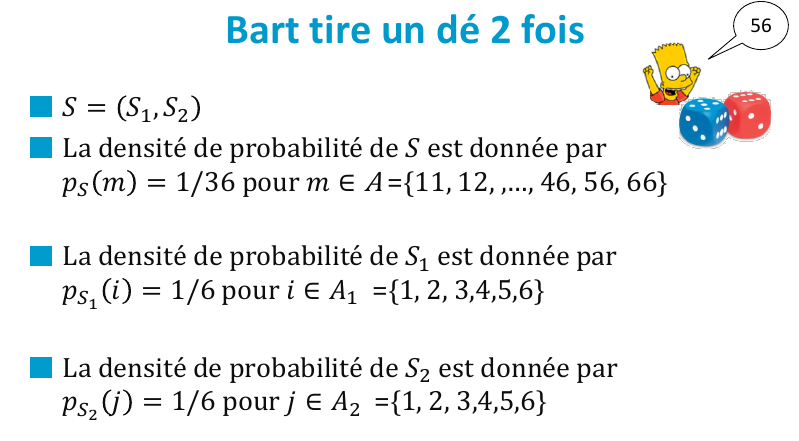
\includegraphics[scale=0.4]{images/bart}
		\caption{Les tirages de Bart}
		\label{bart}
	\end{minipage}
	\begin{minipage}[c]{.46\linewidth}
		\centering
		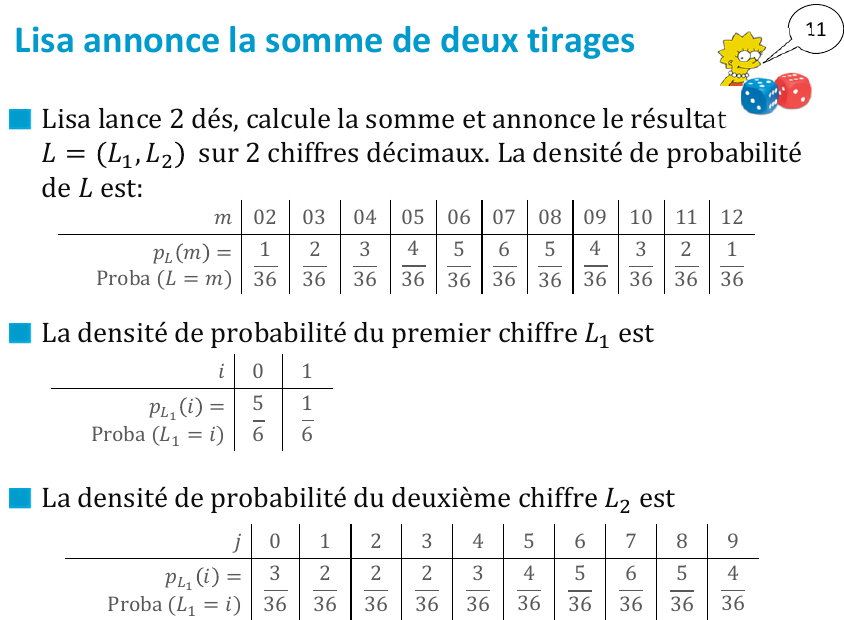
\includegraphics[scale=0.4]{images/lisa}
		\caption{Les tirages de Lisa}
		\label{lisa}
	\end{minipage}
\end{figure}

\subsection{Probabilités}
La \uline{source} S produit un  \uline{message} $m\in A$ (= \uline{Alphabet}). La \uline{probabilité} du message \textit{m} est $0\leq {p(m)} \leq 1$ est définie par $ \frac{\text{cas favorables}}{\text{cas possibles}}$. La fonction $m\to p(m)$ est appelée la \uline{densité de probabilité}. 

Une source composée est 
\begin{equation*}
\overbrace{S}^{\mathclap{\text{source composée}}} =(\underbrace{S_1,S_2,...}_{\mathclap{\text{Sources marginales}}})
\end{equation*}
\begin{exemple}
	Bart tire un dé deux fois. Ainsi $S = (S_1,S_2)$. L'ensemble constitué des deux tirages est une source composée des deux sources marginales, chacun des tirs.\\
	S peut prendre 36 formes : (11,12,13,...,16,21,22,...,66), toutes équiprobables. Ainsi, $p_S(m) = \frac{1}{36}$ pour $m \in \{11,12,...,65,66\}$ et $p_{S_1}(i) = \frac{1}{6} = p_{S_2}(j)$ pour $i,j \in A_1,A_2$ et $A_1 = A_2 = \{1,2,3,4,5,6\}$\\
	\\
	En revanche, Lisa tire deux dés et annonce la somme des tirs. Les densités de probabilités ne sont alors plus équiprobables (probabilité de 7 beaucoup plus grande que celle de 12). Le tableau des probabilités est donné à la Figure \ref{lisa}. De plus, le premier chiffre ne peut être que 0 ou 1 (car les résultats vont de 02 a 12), alors que le second chiffre va de 1 à 9, d'où une certaine inhomogénéité dans les probabilités.
\end{exemple}
\subsubsection{Indépendance}
Deux marginales sont indépendantes ssi, pour tout $i,j$,
\begin{equation*}
	p(S_1 = i,\ S_2 = j) = p(S_1=i)p(S_2=j)
\end{equation*}
\begin{exemple}
	La densité de probabilité de Bart est de $p_S(i,j) = \frac{1}{36}$, alors que la probabilité de ses marginales est de $\frac{1}{6}$. Ainsi, $p_S(i,j) = \frac{1}{36} = \frac{1}{6}\times \frac{1}{6} = p_{S_1}(i)\cdot p_{S_2}(j)$ donc les deux marginales sont indépendantes.\\
	En revanche, pour Lisa, $p_L(1,2) = \frac{1}{36} \neq \frac{0.\overline{3}}{36} = \frac{1}{6}\times \frac{2}{36} = p_{L_1}(1)\cdot p_{L_2}(2)$. Donc les deux marginales ne sont pas indépendantes.
\end{exemple}
\subsection{Entropie}
L'entropie se calcule indépendamment du système de codage (binaire, tertiaire,...). On ne compte que les probabilités d'apparition, pour savoir combien de bits on a besoin au minimum pour représenter nos mots de source.  L'entropie \enquote{encode} tout en binaire, pour mieux les comparer. Changer la base du log servirait à \enquote{encoder} en une autre base. Le calcul de l'entropie est :
\begin{equation}
	H(S) = -\somme{}{s\in A}p(s)\log_2\big(p(s)\big) = \somme{}{s\in A}p(s)\log_2\left(\frac{1}{p(s)}\right)
\end{equation}
\uline{A savoir :} L'entropie est nulle $\iff$ la source est déterministe, c'est à dire \enquote{Il existe un symbole s tel que $p(s) = 1 \iff H(S) = 0$ et pour tous les autres symboles $s' \neq s, p(s') = 0$}\\
\uline{A savoir :} L'entropie est maximale $\iff$ la source est uniforme (= $M\cdot \frac{1}{M}\log_2(M) = \log_2(M)$)\\
\evid{Théorème 1.3:}
\begin{itemize}
	\item $H(S) \leq \log_2(M)$
	\item Les M symboles de la source sont équiprobables $\iff\ H(S) = \log_2(M)$
\end{itemize}

\subsubsection{Indépendance}
Par définition de l'entropie, pour toutes sources composées
\begin{center}
$\begin{array}{ll}
	H(S_1,S_2) \leq H(S_1) + H(S_2)\\
	H(S_1,S_2) = H(S_1) + H(S_2)\text{ Si les sources sont indépendantes (\evid{Théorème 1.4})}
\end{array}$
\end{center}
\begin{exemple}~\\
	\label{H(L2)}
	$\left.\begin{array}{r}
		H(S) = 36\cdot \frac{1}{36} \log_2(36) = \log_2(36) \simeq 5.170 \text{ bits}\\
	H(S_1) = H(S_2) = 6\cdot \frac{1}{6} \log_2(6) = \log_2(6) \simeq 2.585 \text{ bits}
	\end{array}\right\}H(S) = H(S_1) + H(S_2) \\
	\to$ $S_1$ et $S_2$ sont indépendants\\
	Mais\\
	$\left.\begin{array}{r}
		H(L) = \frac{1}{36}\log_2(36) + \frac{2}{36}\log_2(\frac{36}{2}) + ... = 3.27\text{ bits}\\
		H(L_1) = \frac{5}{6}\log_2(\frac{6}{5}) + \frac{1}{6}\log_2(6) = 0.65 \text{ bits}\\
		H(L_2) = \frac{3}{36}\log_2(\frac{36}{3}) + \frac{2}{36}\log_2(\frac{36}{2}) + ... =3.22 \text{ bits}
	\end{array}	\right\} 	H(L) < H(L_1) + H(L_2) = 3.87 \text{ bits} 	 \to L_1$ et $L_2$ sont dépendants
\end{exemple}
\newpage

\section[Codage de Sources]{Chapitre 2 : Codage de Sources}
\subsection{Terminologie}
Le code suivant sert à illustrer la terminologie et à fournir des codes d'exemples.
\begin{figure}[!h]
	\centering
	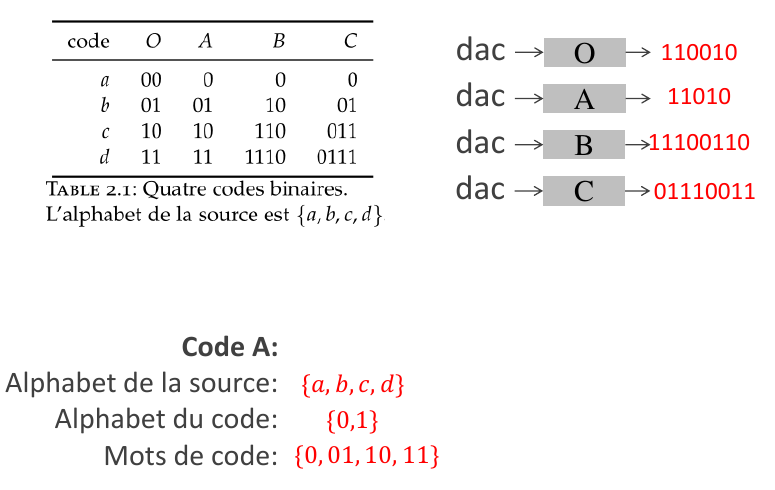
\includegraphics[scale=0.5]{images/terminologie_codage}
	\caption{Terminologie}
	\label{terminologie}
\end{figure}
\subsection{Décodage unique, instantané, arbres}
\subsubsection{Décodage unique}
Un code est à décodage unique si aucune suite de symbole de code ne peut être décodée de 2 manières différentes. 
\begin{exemple}[0.55]
	Par exemple, pour le code A, $bc = 0110 = ada$.
\end{exemple}
 On peut identifier un code comme étant à décodage unique grâce au flair et à quelques outils :
 \setstretch{1}
\begin{itemize}
	\item Tous les mots de code sont de même longueur (c.f. code O)
	\item Un caractère unique marque le début ou la fin de chaque mot (c.f. codes B et C, donc le 0 se trouve uniquement et respectivement à la fin et au début de chaque mot)
	\item S'il est à décodage instantané il est forcément à décodage unique
\end{itemize}
\setstretch{1.2}
\subsubsection{Décodage instantané}
Un code est à décodage instantané si aucun mot de code n'est le préfixe d'un autre (donc si aucun mot n'est dans plus haut dans une même branche de l'arbre de décodage). Simple à vérifier, cela est très pratique. S'il est instantané, alors il est à décodage unique (attention, la réciproque est fausse).
\begin{exemple}
	Les codes O et B sont sans préfixe, alors que les codes A et C ne le sont pas (code A : a est préfixe de b et code C : a est préfixe de tout).
\end{exemple}
\subsubsection{Arbres}
On  construit un arbre en faisant descendre des branches d'un point, chaque branche étant un symbole (0,1 pour un code binaire, 0,1,2 ternaire, etc.) Sa profondeur est la longueur des mots de code (4 dans nos 2 exemples), et à la profondeur $n$ il y aura, pour un code D-aire, $D^n$ mots dans l'arbre complet. 
\begin{figure}[!h]
	\begin{minipage}[c]{0.46\linewidth}
		\centering
		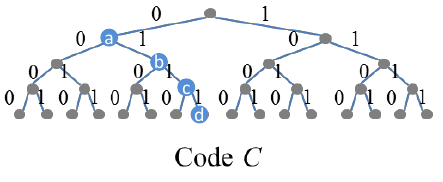
\includegraphics[scale=0.65]{images/arbre_complet}
		\caption{L'arbre complet de C}
		\label{complet}
	\end{minipage}
	\begin{minipage}[c]{0.46\linewidth}
		\centering
		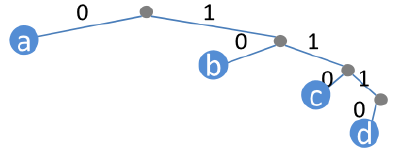
\includegraphics[scale=0.75]{images/arbre_decodage}
		\caption{L'arbre de décodage de B}
		\label{decodage}
	\end{minipage}
\end{figure}\\
Un \evid{arbre complet} (Fig. \ref{complet}) se fait en créant tous les points et toutes les branches\\
Un \evid{arbre de décodage} (Fig. \ref{decodage}) se fait en enlevant les branches en dessous d'un mot de code (\uline{uniquement pour code sans préfixe})


\subsection{Kraft-McMillan}
\subsubsection{Partie 1}
On parle d'un code $\Gamma$ D-aire dont les longueurs des M mots de codes sont $l_1,\ldots,l_M$
\begin{equation}
	\text{Décodage unique} \to \frac{1}{D^{l_1}} + \frac{1}{D^{l_2}} + ... + \frac{1}{D^{l_M}} \leq 1
\end{equation}
Donc si le code est binaire, D = 2. \\
Par contraposée, si l'inégalité n'est pas respectée, alors le code n'est pas à décodage unique. La réciproque est fausse (mais voir la \hyperref[partie 2]{partie 2}).
\begin{exemple}
	L'inégalité de Kraft n'est pas respectée pour A car 
	\begin{equation*}
		2^{-1} + 2^{-2} + 2^{-2} + 2^{-2} = 1.25 > 1
	\end{equation*}
	Donc le code n'est pas à décodage unique. Mais elle l'est pour C car 
	\begin{equation*}
		2^{-1} + 2^{-2} + 2^{-3} + 2^{-4} = 0.9375 \leq 1
	\end{equation*}
	On ne peut cependant pas conclure que C est à décodage unique (démontré avant).
\end{exemple}
\subsubsection{Partie 2}
\label{partie 2}
Même si la réciproque directe est fausse, la seconde partie dit que si des nombres $l_1,...l_M$ satisfont l'inégalité de Kraft, alors un code à décodage instantané est possible avec ces longueurs.
\begin{equation*}
	\frac{1}{D^{l_1}} + \frac{1}{D^{l_2}} + ... + \frac{1}{D^{l_M}} \leq 1 \to \substack{\text{Il existe un code D-aire instantané donc le dictionnaire posède}\\ \text{M mots de code  et dont les longueurs des mots de code sont }l_1,...,l_M}
\end{equation*}
\begin{exemple}
	Même si A n'est pas à décodage unique, en considérant un code A' similaire à A mais ternaire, l'inégalité est respectée, car 
	\begin{equation*}
		3^{-1} + 3^{-2} + 3^{-2} + 3^{-2} = 2/3 \leq 1
	\end{equation*}
	Mais le code n'est toujours pas à décodage unique (toujours parce que $bc = ada$). Nous savons cependant qu'il existe un code avec ces longueurs qui est à décodage unique. Ainsi, en changeant $b = 10$ en $12$, le code est à décodage unique (et même instantané).
\end{exemple}

\subsubsection{Construction d'un arbre de Kraft}
\begin{itemize}
	\item On construit un arbre D-aire de profondeur égal à $l_{\max}$
	\item Placer les mots par ordre croissant
	\item Supprimer les branches en dessous
\end{itemize}
\begin{figure}[!h]
	\centering	
	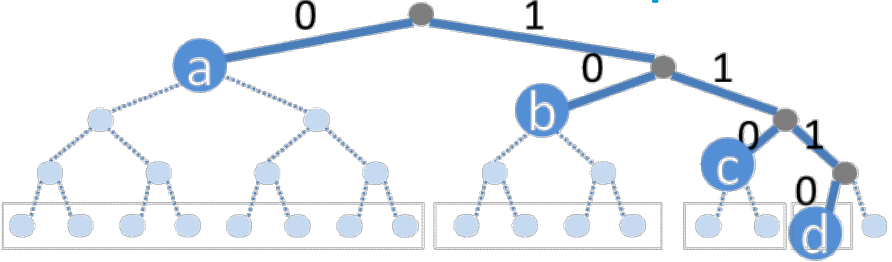
\includegraphics[scale=0.3]{images/arbre_Kraft}
	\caption{Construction de l'arbre de Kraft pour le code B}
	\label{Arbre Kraft}
\end{figure}

\subsection{Définitions, Théorèmes et le reste}

La \evid{longueur} se définit par le nombre de symboles de sources dans un mot de code.\\
L'ensemble des codes respecte ce graphique :
\begin{figure}[!h]
	\centering
	\caption{Ensemble des codes}
	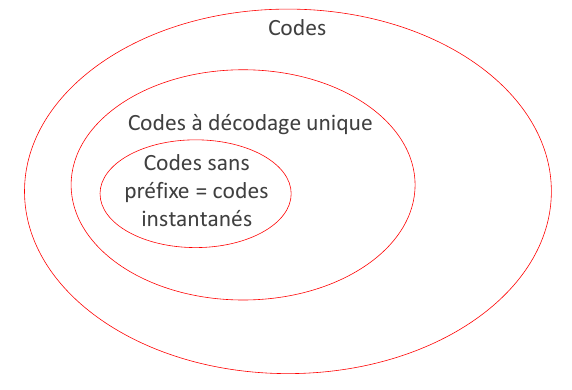
\includegraphics[scale=0.5]{images/tout_code}
\end{figure}\\
De manière similaire à la seconde partie de l'inégalité de Kraft, le \evid{Théorème 2.3} dit que pour tout code à décodage unique, il existe un code à décodage instantané sur les mêmes alphabets de source et de code qui a les mêmes longueurs de mots.
\begin{exemple}[0.7]
	C'est ce qu'on fait en remplaçant le code C par le code B
\end{exemple}

\section[Efficacité d'un Code de Source]{Chapitre 3 : Efficacité d'un code de source}
\subsection{Longueur moyenne}
Pour une Source S, de densité de probabilité \textit{p}, et $\Gamma$ un code D-aire. Alors la longueur moyenne est :
\begin{equation}
	L(\Gamma) = \somme{}{s\in A}p(s)l(\Gamma(s))
\end{equation}
Avec pour unité le \enquote{symbole de code par symbole de source} (Si D = 2 on parle de \textit{bits} par symbole de source)\\
\begin{exemple}~
	\begin{multicols}{2}
		\begin{tabular}{r|c|c|c|c}
			source & a&b&c&d\\
			\hline
			mots de code & 0 & 10 & 110 & 1110\\
			\hline
			p(s) & 0.1 & 0.4 & 0.3 & 0.2 
		\end{tabular} 
		\columnbreak
			
		Avec cette distribution de probabilités, la longueur moyenne est alors \\$L(\Gamma) = 0.1\cdot 1 + 0.4\cdot 2 + 0.3 \cdot 3 + 0.2 \cdot 4 = 2.6$
	\end{multicols}
\end{exemple}

\subsection{Première inégalité de l'entropie}
\label{premiere inegalite entropie}
Pour un code D-aire :
\begin{equation}
	\text{Décodage unique} \to L(\Gamma)\geq \frac{H(S)}{\log_2(D)}
\end{equation}
\subsubsection{Remarques}
Pour un code binaire : $\log_2(D) = 1$, donc l'inégalité deviens $L(\Gamma) \geq H(S)$. Cela se traduit par la remarque suivante  : \uline{On ne peut pas faire mieux que l'entropie}

\subsection{Seconde inégalité de l'entropie}
\label{seconde inegalite entropie}
Un code D-aire de \hyperref[shannon]{Shannon-Fano} doit vérifier 
\begin{equation}
	\frac{H(S)}{\log_2(D)} \leq L(\Gamma_{SF}) < \frac{H(S)}{\log_2(D)}+1	
\end{equation}
\subsubsection{Remarque}
Bien sur, si le code est binaire alors $\log_2(D) = 1$ donc on peut ôter les log de notre équation ; on comprend alors \enquote{Shannon-Fano est entre \enquote{entropie et entropie + 1}}
\subsection{Code/arbre de Shannon-Fano}
\label{shannon}
Données les probabilités d'apparition de chaque mot du dictionnaire, il devient facile de créer un bon encodage :
\begin{enumerate}
	\item On calcule les longueurs de chaque mot avec $\lceil \log_2\left(\frac{1}{p_i}\right)\rceil$
	\item Ça nous donne des longueurs arrondies pour chaque mot.
	\item Ensuite on place dans un arbre, aux bonnes positions
\end{enumerate}
\begin{exemple}
	Prenons un code B' aux probabilités suivantes :
	\begin{tabular}{r|c}
	\hline
	symbole de source & proba\\
	\hline
	$a$ & $0.05$\\
	$b$ & $0.05$\\
	$c$ & $0.1$\\
	$d$ & $0.8$\\
	\hline
	\end{tabular}\\
	Il faut donc que les longueurs des mots de code de Shannon soient les suivantes :  \\
	$a,b : \lceil-\log_2(0.05)\rceil = \lceil4.3219\rceil = 5$\\
	$c : \lceil-\log_2(0.1)\rceil = \lceil3.3219\rceil = 4$\\
	$d : \lceil-\log_2(0.8)\rceil = \lceil0.3219\rceil = 1$\\
	Et depuis là on place dans un arbre aux positions voulues, ce qui donnerait (par exemple) $a = 00001,\ b = 00000,\ c = 0001,\ d = 1$
\end{exemple}

\subsubsection{Remarques} Le code est toujours \enquote{assez bon} mais rarement optimal ; il l'est quand il n'y a pas d'arrondi, donc tous les $p(s)$ sont des puissances de 2 (comme $\frac{1}{2},\frac{1}{4},\frac{1}{8},\frac{1}{16},...$). Ce code est utilisé dans la \hyperref[seconde inegalite entropie]{seconde inégalité de l'entropie}. Le code est instantané.
\begin{exemple}
	Avec la \hyperref[code huffman]{méthode de Huffman}, le code de l'exemple précédent aurait eu des longueurs de respectivement 3,3,2,1, ce qui est plus efficace.
\end{exemple}

\subsection{Code/arbre de Huffman}
\label{code huffman}
 \begin{enumerate}
	\item Placer les mot de code côte à côte triés par probabilités d'apparition
	\item Relier les deux plus faibles probabilités
	\item Additionner leurs probabilités
	\item Recommencer jusqu'à ce que tous soient réunis
\end{enumerate}
\begin{exemple}[0.85]
 	Reprenons les probabilités de notre code B'. La construction se l'arbre de Huffman se trouve à la Figure \ref{arbre huffman bprime}. Nous n'avons alors qu'à lire la position de chaque mot pour trouver son encodage, qui est
 	\setstretch{1}
 	\begin{tabular}{r|l}
 	\hline
 	a & 111\\
 	b & 110\\
 	c & 10\\
 	d & 0\\
 	\hline
 	\end{tabular}
 	\setstretch{1.2}
\end{exemple}
 \begin{figure}[!h]
 	\centering
 	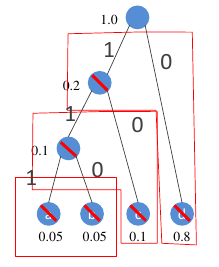
\includegraphics[scale=0.6]{images/arbre_Huffman}
 	\caption{L'arbre de Huffman du code B'}
  	\label{arbre huffman bprime}
 \end{figure}
 
\subsubsection{Remarques} 
\begin{itemize}
	\item 	Le code est optimal : $L(\Gamma_H) \leq L(\Gamma)$ pour tout autre code binaire à décodage unique
	\item 	Le code est instantané
	\item 	Construit un code binaire ! La méthode ne fonctionne a priori pas pour construire un code ternaire ou plus.
\end{itemize} 

\section[Entropie conditionnelle]{Chapitre 4 : Entropie conditionnelle}
\begin{exemple}
	Comme les sources de Bart sont indépendantes, on ne peut pas (pas besoin de) travailler avec l'entropie conditionnelle. En effet, la probabilité de $S_2 = j$ sachant que $S_1 = i$ vaut la probabilité de $S_2 = j$. Par contre le cas de Lisa est plus intéressant, donc c'est sa manière de faire qu'on utilisera dans les exemples, comme à la Figure \ref{conditionnel lisa}
\end{exemple}
\begin{figure}[!h]
	\centering
	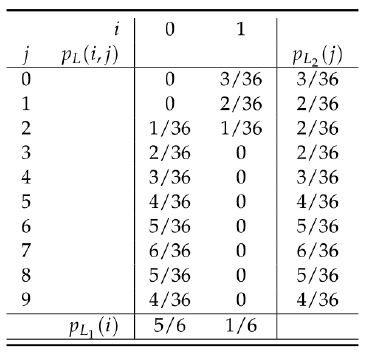
\includegraphics[scale=0.5]{images/entropie_conditionnelle_lisa}
	\caption{Le tableau des probabilités\\ conditionnelles ($L_2|L_1$) de Lisa}
	\label{conditionnel lisa}
\end{figure}
\begin{center}
	\framecolorbox{white}{gray!20}{%
		\begin{minipage}{0.8\textwidth}
	Ce tableau n'est pas simple à lire : la colonne du milieu représente le premier chiffre (qu'on rappelle, est la somme du tirage de deux dés). Les lignes représentent le second chiffre. On a donc aucune chance d'avoir un 0 annoncé en second chiffre si le premier est déjà 0 (elle ne peut pas annoncer 00). Par contre le chiffre 02 a une probabilité 1/36 d'arriver (somme de 1 et 1), et 07 a 6/36 chances d'arriver. 
		\end{minipage}
	}
\end{center}

\subsection{Probabilité conditionnelle}
\enquote{Probabilité que la source $S_2$ émette le symbole $s_2$ sachant que la source $S_1$ émet le symbole $s_1$} $ = p_{S_2|S_1}(s_2|s_1) = \frac{p(s_1,s_2)}{p(s_1)}$
\begin{exemple}
	Probabilité que le second chiffre annoncé soit 2 sachant que le premier est 1 : \[p_{L_2|L_1}(2|1) = \frac{p_{L_1,L_2}(12)}{p_{L_1}(1)} = \frac{\frac{1}{36}}{\frac{1}{6}} = \frac{1}{6}\]
	Et  on voit que cela correspond à la 3\ts{ème} ligne à la colonne \enquote{1} du tableau. En faisant les mêmes calculs pour une autre case, ça fonctionne toujours (par exemple $p_{L_2|L_1}(2|0) = \frac{1}{30}$)
\end{exemple}

\subsection{Entropie conditionnelle}
L'entropie conditionnelle de $S_2$ sachant $S_1 = s_1$ est l'entropie de la densité conditionnelle de $S_2$ sachant $S_1 = s_1$ :
\begin{equation}
	H(S_2|S_1 = s_1) = -\somme{}{s_2 \in A_2} p_{S_2|S_1}(s_2|s_1)\log_2\big(p_{S_2|S_1}(s_2|s_1)\big) 
	\label{pour un s1}
\end{equation}
\begin{exemple}
	\begin{align*}
	H(L_2|L_1 = 1) = \frac{3}{6}\log_2\(\frac{6}{3}\) + \frac{2}{6}\log_2\(\frac{6}{2}\) + \frac{1}{6}\log_2\(\frac{6}{1}\) \approx 1.459 \text{ bits} \\
	H(L_2|L_1 = 0) = \frac{1}{30}\log_2\(\frac{30}{1}\) + \frac{2}{30}\log_2\(\frac{30}{2}\) + \ldots + \frac{4}{30}\log_2\(\frac{30}{4}\) \approx 2.857 \text{ bits}
	\end{align*}
\end{exemple}
Et l'entropie (générale, pas dans un cas) conditionnelle de $S_2$ sachant $S_1$ en est la moyenne :
\begin{equation}
	H(S_2|S_1) = \somme{}{s_1\in A_1} H(S_2|S_1=s_1)p_{s_1}(s_1)
	\label{pour tout s1}
\end{equation}
\begin{exemple}
	Rappelons que la probabilité que le premier chiffre soit 0 est de 5/6 et qu'il soit 1 est de 1/6. Ainsi :
	\[H(L_2|L_1) = \frac{1}{6}H(L_2|L_1=1) + \frac{5}{6}H(L_2|L_1=0) = \frac{1}{6}1.459+ \frac{5}{6}2.587 = 2.624 \text{ bits}\]
	Nous avons vu à l'exemple \ref{H(L2)} que $H(L_1) = 0.65$. Or, $H(L_1) + H(L_2|L_1) = H(L_1,L_2)$ (c.f. la \hyperref[enchainement]{règle de l'enchaînement})
\end{exemple}
Cela s'interprète comme étant la \uline{quantité d'information moyenne supplémentaire}, la quantité d'information reçue en observant $S_2$ après avoir observé $S_1$.\\
\begin{exemple}
	Le point à bien saisir ici, c'est que l'équation \eqref{pour un s1} regarde dans un cas précis ; pour reprendre les tirages de Lisa, cette équation doit se faire beaucoup de fois : par exemple, quelle est l'entropie du second chiffre \textit{sachant que le premier est 0.}
	
	L'équation \eqref{pour tout s1} regarde la moyenne de tous les cas : quelle est l'entropie du second chiffre de Lisa \textit{en admettant que je connaisse le premier}
\end{exemple}

\subsubsection{Règle de l'enchaînement}
\label{enchainement}
Pour une source composée :\\
$\begin{array}{ll}
	H(S_1,S_2) 	&= H(S_1) + H(S_2|S_1)\\
				&= H(S_2) + H(S_1|S_2)
\end{array}$\\
(Donc information totale = information d'un + l'information supplémentaire)\\
Peut aussi dans l'autre sens ($H(S_2|S_1) = H(S_1,S_2) - H(S_1)$)

\subsubsection{Conditionner réduit l'entropie}
Pour une source composée :\\	
$\begin{array}{ll}
	H(S_2|S_1) \leq H(S_2) 	&\\
	H(S_2|S_1) = H(S_2) &\text{ si et seulement si $S_1$ et $S_2$ sont indépendants}
\end{array}$

\subsection{Remarques, définitions, théorèmes}
Une source est fonction d'une autre si connaître le premier implique le second. Par exemple, tirer deux dés ($S_1, S_2$) et calculer leur somme $K$. $K$ est alors \uline{fonction de ($S_1,S_2$)}, car \textit{K}, n'apporte aucune information supplémentaire par rapport à ($S_1,S_2)\ \Rightarrow\ S_2$ est \textit{fonction} de $S_1$ si $H(S_2|S_1) = 0$

\section[Théorème du Codage de Sources]{Chapitre 5 : Théorème du Codage de Sources}
\paragraph{Note personnelle}
Ce chapitre est vraiment très compliqué (à mon goût le plus difficile), les définitions sont floues et la série avec était horrible ; il est donc difficile de retranscrire toute la matière sans la recopier mot-à-mot. Une partie essentielle de la compréhension est passée par les question avec clickers. Je vous conseille pour ce chapitre de vraiment relire les slides et le livre, mon résumé ne transmettant que peu ce qui est transmis dans le cours. Refaire/lire la série 4 et son corrigé est une bonne idée aussi.

\subsection{Définitions, théorèmes}
\evid{Bloc :} Un bloc produit une suite de \textit{n} symboles venant chacun de l'alphabet A. L'alphabet de $S^n$ est $A^n$\\
\\
\evid{Source étendue :} Une source étendue est un bloc infini. Pour le vérifier, il faut vérifier 2 points précis :
\begin{itemize}
	\item   $S^n$ est une source à \textit{n} composantes, sur l’alphabet $\underbrace{A \times A \times \ldots \times A}_{\times n}$; notons $p_{S^n}$ sa densité de probabilité.
	\item La densité de probabilité de la source constituée des \textit{n} premières sources marginales de $S^{n+k}$ est égale à $p_{S^n},\ \forall k,n \geq 1$
\end{itemize}
Si ces deux items sont respectés, la source est étendue.\\
\\
\evid{Source stationnaire} Pour qu'une source soit stationnaire, il faut vérifier si la densité de probabilité $p_{S_{k+1},S_{k+2},...,S_{k+n}}(s_1,s_2,...,s_n)$ est la même pour toutes les valeurs de $k\geq 0$. Autrement dit, le fait de regarder la densité de probabilité d'un bloc de longueur \textit{n} (fixe par cas), ne devrait pas changer, quel que soit l'endroit où on regarde (par exemple regarder tous les bloc de taille 20 ; regarder au 3\ts{ème} ou 1000\ts{ème} tirage ne devrait rien changer). Pour cela, il faut calculer la probabilité (de longueur n) du bloc ; si la probabilité dépend d'un k, alors la source n'est pas stationnaire.\\
\\
\evid{Entropie \uline{d'un} symbole :} $H(S) = \limite{n \to +\infty} H(S_n)$ (attention, entropie du n\ts{ème} symbole, pas du bloc de taille n)\\
\evid{Entropie \uline{par} symbole :} $H^*(S) = \limite{n\to +\infty} H(S_n | S_1,S_2,\ldots,S_{n-1})$\\
\\
\evid{Source régulière :} Une source est régulière si les limites $H(S)$ et $H^*(S)$ existent et sont finies\\
\\
\evid{Bits par symboles} ($\neq$ entropie par symbole) : $\frac{L_n}{n}$\\
\\
\evid{Entropie d'un bloc} Soit S source étendue régulière, on peut poser que $\limite{n\to +\infty}\frac{H(S_1,S_2,...,S_n)}{n} = H^*(S)$\\
\\
\evid{Théorème 5.3 : (Codage de Source)} Soit $S$ une source étendue régulière et $H^*(S)$ son entropie par symbole. Soient $L^n_{SF}$, respectivement $L^n_{H}$, les longueurs moyennes des codes D-aires de Shannon-Fano, respectivement Huffman, pour un bloc de n symboles de la source. Alors
\begin{equation*}
	\limite{\ninf} \frac{L_H^n}{n} = \limite{\ninf} \frac{L_{SF}^n}{n} = \frac{H^*(S)}{\log_2(D)}
\end{equation*}
Autrement, pour une source régulière et un code optimal, la longueur moyenne divisée par la taille du bloc n'est autre que l'entropie par symbole.\\
Notons que cela implique une chose intéressante : \uline{Pour un code binaire :} $\limite{\ninf} \frac{L_H^n}{n} = H^*(S)$\\
\evid{Définitions :}
\begin{itemize}
	\item Toutes les sources stationnaires sont régulières
	\item \evid{Théorème 5.1 :} Pour une source régulière, $H^*(S) \leq H(S)$ (si les sources marginales sont indépendantes, alors il y a égalité)
\end{itemize}

\subsection{Rapport de compression}
\begin{wrapfigure}{l}{8.5cm}
	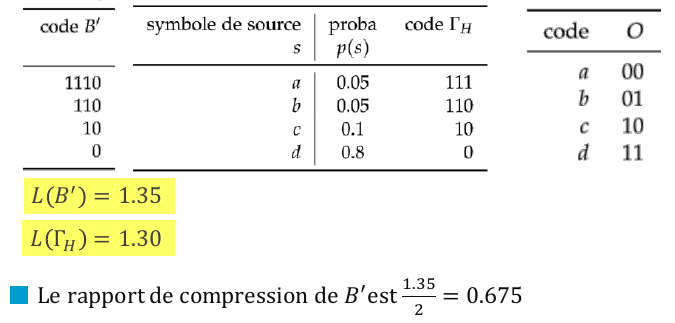
\includegraphics[scale=0.5]{images/compression}
	\caption{Un exemple de code}
	\label{compression}
\end{wrapfigure}
Le rapport de compression d'un code se calcule en divisant sa longueur moyenne par la longueur moyenne d'un code \enquote{stupide}, (un code de longueur constante la plus petite possible), obtenu par \[n\lceil \log_2(M)\rceil\]. Cela nous donne que le rapport de compression est \[\frac{L^n}{n\lceil \log_2(M)\rceil} (\leq 1)\]
Dans l'exemple de la Figure \ref{compression}, le code O est le code stupide. Sa longueur est de 2, raison pour laquelle on divise la longueur moyenne de B' par 2\\
Nous savons aussi, grâce aux entropies, que le rapport de compression d'un code optimal est \[ \sim\frac{H^*(S)}{\log_2(D)}\]

\subsection[Récapitulation types sources]{Régulière, stationnaire, étendue : quoi et pourquoi ?}
\begin{itemize}
	\item \evid{Régulière} : On a vu l'importance de $H(S_n)$ et de $\frac{H(S_1,...,S_n)}{n}$. On aimerait savoir si, pour la source donnée, ces quantités se stabilisent pour $n$ assez grand. C'est le cas des sources régulières.
	\item \evid{Stationnaire} : Pour la plupart des sources, les propriétés statistiques ne dépendent pas d'un \enquote{décalage d'indexation}.
			\begin{exemple}
				Si on observe \[[...]101101[...]\] est-ce une réalisation de \[[...]S_1S_2S_3S_4S_5S_6[...]\] ou de \[[...]S_{n+1}S_{n+2}S_{n+3}S_{n+4}S_{n+5}S_{n+6}[...] ?\]
				Aucune différence statistique si stationnaire
			\end{exemple}
	\item 	\evid{Étendue} :On nous donne une \textit{famille} de sources. Cela forme-t-il une source étendue $S_1,S_2,S_3,...$ ?
			\begin{exemple}
				Prochaine nouveauté, le display triangulaire : le iDisplay (Figure \ref{etendue}). Cela ne donne pas une source étendue, car \[\begin{array}{ll}
					\somme{}{i\in \text{ couleurs}} \overbrace{P_{S^2}(\text{vert}, i)}^0 & = 0\\
						& \neq P_{S^1}(\text{vert}) = 1
				\end{array}
				\]
				Dit autrement, $S_2$ n'est pas une source étendue du type $(S^1,S^2)$ etc.
			\end{exemple}
\end{itemize} 			
\begin{figure}[!h]
	\centering
	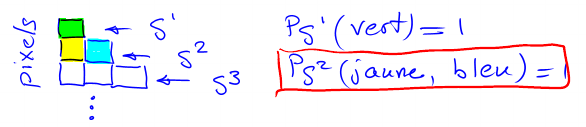
\includegraphics[scale=0.5]{images/etendue}
	\caption{}
	\label{etendue}
\end{figure}

\subsection[Ne pas Confondre]{Ne pas confondre, pour un code binaire}
\[\text{Rapport de compression } = \frac{L^n}{n\lceil \log_2 M\rceil} \neq \frac{L^n}{n} = \text{ bits pas symbole}\]
même si leur valeur est identique, car le code est binaire
\newpage

\section[Cryptographie]{Chapitre 6 : La cryptographie}
En cryptographie nous avons essentiellement 2 types d'encodage : symétrique et asymétrique. Le codage symétrique a l'avantage d'être presque incassable (alors que l'asymétrique est sujette à plus d'attaques), mais le transfert de la clé secrète est difficile. Si on a la clé on peut tout savoir ; la difficulté devient alors de transmettre cette clé sur un canal sécurisé. Le cryptage asymétrique utilise en revanche une clé secrète et une clé publique.
\subsection{Terminologie}
\begin{multicols}{2}
	\begin{itemize}
		\item 	\textit{P} : le \textit{Plaintext}, le texte en clair, celui de départ.
		\item 	\textit{C} : le \textit{cyphertext}, le texte codé, celui que l'on transmet (qui risque d'être intercepté).		
		\item 	\textit{K} : la clé (\textit{Key}) de cryptage.
		\item	\textit{k} : la clé de décryptage 
		\item 	$E_k(P)$ : l'\textit{Encodage} qui utilise la clé \textit{k} pour encoder P. C'est la fonction de \textit{P} à \textit{C}.
		\item 	Symétrique : Si \textit{K} = \textit{k}. On garde alors cette clé secrète, et il faut décrypter d'un autre moyen (par exemple brute-force, ou convenu longtemps à l'avance).
		\item 	Asymétrique : Si \textit{K} $\neq$ k. À ce moment, soit on rend \textit{K} publique et on garde $k$ secrète (confidentialité) soit l'inverse (authentification)
	\end{itemize}
\end{multicols}
Par principe, nous devons supposer que l'intrus intercepte tout, comme notre destinataire, qu'il l'intercepte à la transmission (le message est alors codé), et qu'il sait quelle méthode a été utilisée (se baser sur le manque de connaissance de l'intrus est extrêmement risqué et ne constitue pas une sécurité à long terme).
\subsection{Chiffre de César}
Cryptage symétrique. On prend un chiffre (modulo 26), et on décale les lettres P de cet ordre. 
\begin{exemple}[0.65]
	Par exemple, si K = 3, alors $A \to D, B\to E,...,Z\to C$
\end{exemple}
Cryptage facile à faire mais élémentaire à briser de façon brute-force (il n'y a que 26 décalages possibles ; tous les essayer se fait très rapidement).
\subsection{Substitution monoalphabétique}
On définit une table de remplacement unique (chaque lettre claire a une et une seule lettre codée). Cette propriété garantit le décodage unique. Briser ce code est un peu plus difficile ; on peut chercher dans un texte codé la lettre la plus fréquente, qui correspond sûrement à un \textit{e} (la lettre la plus fréquente en français). On peut aussi chercher des mots en rapport (si c'est commercial chercher le mot \textit{vendre}, ou \textit{action}). L'attaque exhaustive est longue à la main ($26!$ possibilités), mais peut se faire rapidement avec un ordinateur.
\subsection{Chiffre de Vigenère}
Cryptage symétrique, substitution polyalphabétique. On choisit un mot/phrase. On associe à chaque lettre un chiffre (A=0, Z=25); on aligne ensuite P avec des répétitions de K, et on décale la position des lettres de P d'autant. En calcul, on peut simplement faire $(P+K)\mod 26$ \\
Par exemple, avec la clé BONJOUR (associée aux chiffres 1,14,13,914,20,17): \\
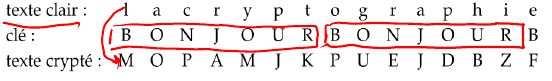
\includegraphics[scale=0.7]{images/vigenere}\\
Il y a $26^n$ clés (avec \textit{n} la taille de K)$\to$ attaque exhaustive difficile. Si la clé est courte et le texte est long, il est possible de faire des attaques basées sur la la fréquence des lettres.
\subsection{Chiffre de Vernam}
\begin{wrapfigure}{r}{3.2cm}
	\centering
	\captionsetup{justification=centering}
	\begin{tabular}{c|cc}
		xor & 0 & 1\\
		\hline
		0 & 0 & 1\\
		1 & 1 & 0
	\end{tabular}
	\caption{\\La table du xor}
	\label{xor}
\end{wrapfigure}
Cryptage symétrique. On parle d'un masque \textit{jetable}, ou \textit{à usage unique}(one time pad). On doit avoir \textit{K} et \textit{P} de même longueur. On calcul ensuite \textit{C} par \fbox{$P \bigoplus K$} (xor, défini parle tableau de la Figure \ref{xor}) . Il faut la clé et le texte soient indépendants (par exemple faire un lancer de dés pour déterminer \textit{K})\\
Le décodage se fait par \fbox{$P = C \bigoplus K$}. Ce système est a confidentialité parfaite (pour autant que \textit{P} et \textit{K} sont indépendants)
\begin{exemple}
Soit notre clé K = 1101 et notre texte P = 0100. C se trouve de cette manière :
\begin{tabular}{c c}
	& 0100\\
	$\bigoplus$ & 	1101\\
	\hline
	= & 1001
\end{tabular}
Donc $C = 1001$. Le décryptage se fait de la même manière : 
\begin{tabular}{c c}
	& 1001\\
	$\bigoplus$ & 	1101\\
	\hline
	= & 0100
\end{tabular} et on retrouve P 	
\end{exemple}
\subsection{La confidentialité parfaite}
Un système est à confidentialité parfaite si connaître \textit{C} ne dit absolument rien sur \textit{P} (nous supposons que l'intrus connaît la méthode de chiffrement utilisée). 
\begin{exemple}
	Prendre \textit{P} et \textit{K} deux chiffres de 1 à 7, et les multiplier pour donner \textit{C} n'est pas à confidentialité parfaite : Si \textit{C} = 49, alors \textit{P} = \textit{K} = 7
\end{exemple}
Par le \evid{Théorème 6.2} : Nous prenons un texte à confidentialité parfaite. Si la clé et le texte clair sont choisit indépendamment, alors 
\begin{equation*}
	H(P) \leq H(C) \leq H(K)
\end{equation*}

\section[Arithmétique Modulaire]{Chapitre 7 : Arithmétique Modulaire}
\subsection{Division Euclidienne}
Pour tout $a,b$, des entiers, il existe un couple $q,r$ tels que $a = bq + r$ (avec q = quotient et r = reste et $0 \leq r \leq |b|-1$). 
\begin{exemple}[0.7]
	Pour $a = 23$ et $b = 5$, alors $q = 4,\ r = 3$, car $23 = 5\cdot 4 + 3$.
\end{exemple}  Notons que l'on peut calculer (si $b > 0$) : $q = \lfloor\frac{a}{b}\rfloor,\ r = a-bq$. On dénote r comme étant $a \mod b$ (reste du modulo-division entière de a par b)
\subsection{La congruence modulo}
Deux entiers \textit{a} et \textit{b} sont \enquote{congru modulo \textit{m}} si ils ont le même reste dans la division par m, et l'on écrit 
\begin{equation*}
	a\equiv b\ (\text{mod } m)
\end{equation*}
\begin{exemple}[0.45]
	 $\quad 33 \equiv 23 \equiv 13 \equiv 3 \text{ (mod } 10)$
\end{exemple}
\begin{itemize}
	\item On dit que \textit{x} est divisible par \textit{m} si $x \equiv 0 ( \mod m)$
	\item Tout nombre est congru modulo $m$ à son reste dans la division par $m$
	\item En général, $x\equiv y (\mod a) \iff (x-y) \equiv 0 (\mod a)$
\end{itemize}
\subsubsection{Relation d'équivalence}
La congruence modulo est une relation d'équivalence sur \Z, donc :
\begin{multicols}{2}
	\begin{itemize}
		\item 	Réflexivité : $a \equiv a (\mod m)$
		\item 	Symétrie :\\ $a \equiv b (\mod m) \iff b \equiv a (\mod m)$
		\item 	Transitivité : Si $a \equiv b (\mod m)$ et \\$b \equiv c ( \mod m)$ alors $a \equiv c (\mod m)$
	\end{itemize}
\end{multicols}
De plus, par le théorème de l'arithmétique modulaire :
Si $a \equiv a' (\mod m)$ et $b \equiv b' (\mod m)$, alors
\begin{align*}
	a+ b \equiv a' + b' (\mod m)\\
	ab \equiv a'b' (\mod m)\\
	a^n \equiv  a'^n (\mod m)
\end{align*}
\subsubsection{Calculs/trucs}
Il est depuis là facile de faire des calculs ; par exemple, $2^{1000}$ est-il divisible par 3 ? Nous savons que $2^{1000} \equiv (-1)^{1000} \equiv 1 \mod 3$. Donc ça n'est pas divisible par 3.

De même, $37^{9876543}$ est il multiple de 7 ? $37^{9876543} \mod 7 = 2^{9876543} \mod 7 = 	(2^3)^{\frac{9876543}{3}} \mod 7 = 8^{3292181} \mod 7 = 1^{3292181} \mod 7 = 1 \mod 7 = 1$

Il est aussi facile de calculer le reste de la division par 2 : Si le dernier chiffre est pair le reste est de 0 ; en revanche, il  est de 1 si le chiffre est impair.

Finalement, le calcul du reste de la division par 9 se fait en divisant \textit{la somme des chiffres qui composent le nombre} par 9. Ainsi, $1234567890 \mod 9 = 1+2+3+4+5+6+7+8+9+0 \mod 9 = 45 \mod 9 = 4+5 \mod 9 = 9 \mod 9 = 0$

Notons aussi que les calculs se font normalement aussi sur les modulo. Seule la division ne se fait pas normalement. Pour ça, on peut changer \enquote{mod} en \enquote{bq + r}, afin de pouvoir faire les calculs normaux.
\subsection{Procédure MOD 97-10}
Utilisée essentiellement par les banques, comme numéro de contrôle ; une erreur courante est d'inverser 2 chiffres, donc ajouter ce chiffre de contrôle permet de repérer l'immense majorité des erreurs.

Pour ce faire, il faut prendre notre chiffre bancaire, ajouter 00 à la fin, calculer le \textit{r} = numéro mod 97. Ensuite, remplacer le 00 par \fbox{98-r}\footnote{98 et non pas 97, afin que le mod du nouveau chiffre fasse 1 et pas 0}. Ce nouveau chiffre doit être congru à 1 modulo 97.

Notons que dans les numéros IBAN, nous avons 2 lettres et 2 chiffres. Les 2 lettres sont remplacées par un numéro à 4 chiffres ($A\to 10,...,Z\to 35$). On met ce numéro (et les 2 chiffres de contrôle) à la fin, et le calcul se fait là-dessus.

En gros :
\begin{enumerate}
	\item 	Ajouter 00 à la fin
	\item 	r = reste de la division par 97
	\item 	Chiffre de contrôle $c = 98-r$; remplacer 00 par $c$
	\item 	Vérification : le mot reçu doit être $\equiv 1 (\text{mod }97)$
\end{enumerate}

\begin{exemple}[0.55]
	\setstretch{1}~
	\begin{enumerate}
		\item 	$x = 212351234$\textcolor{red}{00}
		\item 	21235123400 $\equiv$ 91 (mod 97) $\to r = 91$
		\item 	$c = 98-r = 98-91 = 07$
		\item 	Le chiffre avec chiffres de contrôle : 212351234\textcolor{red}{07}
	\end{enumerate}
\end{exemple}
\setstretch{1.2}
\subsection{Décomposition en nombres premiers}
\setstretch{1}
\begin{itemize}
	\item 	Premier théorème : Pour tout entier a positif, il existe une suite d'entiers $p_1<p_2<...<p_k$ et une suite unique d'exposants $\alpha_1>0,...,\alpha_k>0$ tels que
			\begin{equation*}
				a = p_1^{\alpha_1}\cdot...\cdot p_k^{\alpha_k}
			\end{equation*}
			Les nombres $p_1,...,p_k$ sont appelés les facteurs premiers.
	\item 	Un entier ($\in \Z$) est premier s'il n'est divisible que par 1 et lui-même.
	\item 	Soient 2 entiers a et b. a divise b si et seulement si tous les facteurs premiers de a apparaissent dans la décomposition de b, à une puissance égale ou supérieure.
	\item 	Le PGCD : on décompose les deux chiffres, et on prend tout ce qui est en commun ; si un facteur apparaît 2x, on le prend à la plus petite puissance (car cette puissance est en commun).
	\item 	Deux nombres sont premiers entre eux si et seulement si leur pgcd est de 1 (aucun facteur premier en commun)
	\item 	Deux nombres premiers sont premiers entre eux.
	\item 	Pour un entier a et un premier p tels que $1\leq a \leq p-1$, alors a et p sont premiers entre eux
	\item 	Soient a et b deux entiers premiers entre eux, et c un entier. Si a et b divisent c, alors ab divise c.
\end{itemize}
\setstretch{1.2}

\section{Arithmétique modulaire Z/mZ}
\subsection{Classe de congruence}
Pour $m \geq 2$ (le module) un entier fixé. Pour tout entier $a$, on appelle \uline{classe de congruence} de $a$ modulo $m$ ($[a]_m$) tous les entiers $a'$ tels que $a \equiv a' (\mod m)$	. L'ensemble des classe de congruence modulo m s'écrit $\Z/m\Z$

La somme et le produit se font instinctivement : $[a]_m + [b]_m = [a+b]_m,\quad [a]_m \cdot [b]_m = [ab]_m$
L'addition se fait normalement (transitivité, commutativité, associativité, élément neutre et symétrique). La multiplication aussi, sauf pour l'élément inverse.
\subsection{Notation}
\begin{itemize}
	\item 	$k[a]_m = [k]_m[a]_m = [ka]_m$
	\item 	$-[a]_m = [-a]_m =[-a + km]_m$
\end{itemize}
\subsection{L'inverse}
$[a]_m$ possède $[b]_m$ comme inverse si $[a]_m[b]_m = [1]_m$. L'inverse est alors noté $([a]_m)^{-1}$\\
\evid{Attention !} Il est possible qu'un entier n'ait pas d'inverse. Par exemple, $[2]_4$ n'est pas inversible.
\subsubsection{Remarques}
\begin{itemize}
	\item 	$[0]_m$ n'a jamais d'inverse
	\item	S'il existe, l'inverse est unique
	\item 	$([a]_m)^k = \overbrace{[a]_m\cdot [a]_m \cdot ... \cdot [a]_m}^{k\times} = [a^k]_m$
	\item 	Pour \textit{p} un premier, tous les nombres de $\Z/p\Z$ sont inversibles (sauf $[0]_p$ bien sûr)
	\item 	Selon Euclide et Bézout, $[a]_m$ est inversible si et seulement si $a$ et $m$ sont premiers entre eux.
\end{itemize}

\subsection{Algorithme d'Euclide}
Soient $a$ et $b$ deux entiers, avec $b\neq 0$, et soit $a = bq + r$. Alors 
\begin{equation*}
	pgcd(a,b) = pgcd(b,r)
\end{equation*}
\uline{Exemple :}\\
$pgcd(122,22) = pgcd(22,12) = pgcd(12,10) = pgcd(10,2) = pgcd(2,0) = 2$	
\subsection{L'identité de Bézout}
Soient a et b deux entiers ; il existe $u$ et $v$ entiers tels que $au + bv = pgcd(a,b)$

\subsection{Inverser un chiffre}
L'algorithme ci-dessous permet de calculer l'inverse d'un nombre dans une base donnée. Difficile de le faire en mots, le mieux est avec un exemple :
\begin{exemple}
	Cherchons l'inverse de 9 dans la base 95 :\\
	$\begin{array}{l}
	\fbox{95} = 10\cdot \fbox{9} + 5 \iff \fbox{95} - 10\cdot\fbox{9} = 5 \curvearrowright \\
	\fbox{9} = 5 + 4   \iff \fbox{9} -5 = 4 = \fbox{9} - (\fbox{95} - 10\cdot\fbox{9}) = 11\cdot\fbox{9} - \fbox{95} = 4\\ 
	5 = 4 + 1 \iff 5 - 4 = 1 =\(\fbox{95}-10\cdot\fbox{9}\) - \(11\cdot\fbox{9}-\fbox{95}\) = 2\cdot\fbox{95}-21\cdot\fbox{9}
	\end{array}$\\
	Donc nous avons montré que \[1 = 2\cdot 95 - 21\cdot 9 = \underbrace{[2\cdot 95]_{95}}_0 - [21\cdot 9]_{95}\] et ainsi également que \[[-21]_{95}\cdot[9]_{95} = [1]_{95}\]
	et donc l'inverse de 9 est logiquement 
	\[[-21]_{95} = [95-21]_{95} = [74]_{95}\]
\end{exemple}
\section{Chapitre 9 : Algèbre abstraite}
\subsection{Notation}
\begin{itemize}
	\item $e$ = élément neutre
	\item $\varphi(m)$ = indice d'Euler (de $m$)
	\item $\star$ une opération, définie mais quelconque.
\end{itemize}

\subsection{Groupe commutatif}
Soit $(G,\star)$ un ensemble G muni de l'opération binaire $\star$. C'est à dire un mécanisme qui associe à deux éléments $a$ et $b$ de G (distincts ou non) un élément de G noté $a\star b$. 

$(G,\star)$ est appelé un \uline{groupe commutatif} (ou groupe abélien) s'il possède les propriétés :

\setstretch{1}
\begin{itemize}
	\item 	\uline{Associativité} 	$a\star (b\star c) = (a\star b)\star c$
	\item 	\uline{Neutre} il existe un $e$ tel que $a\star e = e\star a = a$
	\item 	\uline{Symétrique} pour tout élément $a$, il existe un $a'$ tel que $a \star a' = e$
	\item 	\uline{Commutativité} $a\star b = b\star a$
\end{itemize}
\setstretch{1.2}

\subsubsection{Groupe modulaire multiplicatif}
On connaît déjà $\Z/m\Z$ qui représente tous les entiers de classe m. 

Maintenant nous considérons \uline{$\Z/m\Z^*$}, qui est l'ensemble des éléments inversibles de $\Z/m\Z$ (donc ceux qui sont plus petits que $m$, et premier avec lui).

\subsection{Produit cartésien}
$(\Z/2\Z) \times (\Z/5\Z)$ donnera $(00), (01), (02), (03) ,(04), (10), (11), (12), (13), (14)$. On calcule symbole par symbole (donc le second se calculera mod 5 alors que le premier se calculera mod 2). On peut faire autant de multiplications qu'on veut. Si $(G,\star)$ et $(H.\star)$ sont des groupes, alors $(G\times H,\star)$ est aussi un groupe.

\subsection{Isomorphisme}
Deux groupes sont isomorphes si on peut renommer les éléments de manière à ce que les tableaux correspondent.

\subsection{Période d'un élément}
Soit $(G,\star)$ un groupe commutatif fini (doté d'un élément neutre).
\begin{enumerate}
	\item Pour tout élément $a \in G$, il existe un entier $k \geq 1$ tel que $\overbrace{a\star a \star \ldots \star a}^{k\times} = e$. Le plus petit de ces entiers est appelé la \uline{période de $a$}.
	\item Pour tout entier positif $l,\ \overbrace{a\star a\star a \star...\star a}^{l\text{ fois}} = e$ si et seulement si la période divise $l$ ; autrement dit, la période de chaque éléments de G divise le nombre d'éléments du groupe.
\end{enumerate}
\begin{exemple}[0.85]~\\
	Dans $(\Z/12\Z,+)$, la période est le plus petit élément entier positif $k$ tel que $k[a]_{12} = [0]_{12}$\\
	Dans $(\Z/12\Z,\cdot)$, la période est le plus petit élément entier positif $k$ tel que $([a]_{12})^k = [1]_{12}$
\end{exemple}
\evid{Théorème 9.3} (Lagrange) Soit $(G,\star)$ un groupe commutatif fini, de cardinal $n$. La période de tout élément de $G$ divise $n$.

En particulier, notons $e$ l'élément neutre de G. Pour tout $a  \in G$ : \[\overbrace{a\star a \star a \star...\star a}^{n\times} = e\]

De ce théorème important découle ce corollaire :\\
\evid{Corollaire 9.4 (Théorème d'Euler}. Nous posons $\varphi(m)$ (\uline{l'indicatrice d'Euler}), qui est le nombre d'éléments (le cardinal) de $\Z/m\Z^*$.  Alors, pour tout entier positif $m$ et tout entier $a$ premier avec $m$ :
\[([a]_m)^{\varphi(m)} = [1]_m\]
ou encore
\[a^{\varphi(m)} \equiv 1 (\text{mod }m)\]
\newpage

\subsection{Restes chinois, l'application $\psi$}
\begin{wrapfigure}{r}{4cm}
	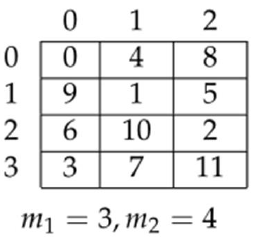
\includegraphics[scale=0.5]{images/chinois}
	\caption{Remplissage d'une boîte de $3\times 4$}
	\label{chinois}
\end{wrapfigure}
Tiré du jeu des restes chinois : on remplit par la diagonale une boite torique\footnote{une fois sorti de la boite, on continue à la manière d'une sphère, donc en haut si on finit en bas, à gauche si on finit à droite}. Dans certains cas la boite se remplit sans problème, dans d'autres elle \enquote{bouclera} (des cases seront remplies plusieurs fois, d'autres jamais). Mathématiquement, cela revient à calculer le modulo selon le nombre de ligne et de colonnes et les placer aux coordonnées indiquées. 
\begin{exemple}[0.7]
Exemple : Avec $m_1$ le nombre de colonnes et $m_2$ le nombre de lignes, placer un chiffre $k$ dans la boite le place aux coordonnées $[k]_{m_1},[k]_{m_2}$. Dans la boite de la Figure \ref{chinois} 7 ira à la position $([7]_{3},[7]_4) = (1,3)$, donc à la colonne 1, ligne 3
\end{exemple}
Cela nous permet de comprendre un point essentiel : Cette boîte se remplira complètement (sans bouclage) si et seulement si les  entiers $m_1$ et $m_2$ sont premiers entre eux.

\subsubsection{Le théorème}
L'application $\psi$ est définie comme telle :
\[\psi : \left\{\begin{array}{l}
	\Z/m_1m_2\Z \to \Z / m_2 \Z \times \Z / m_2 \Z \\
	{}[k]_{m_1 m_2} \to ([k]_{m_1},[k]_{m_2})
\end{array}\right.\]
Si $m_1,m_2$ sont premiers entre eux, l'application est bijective et représente un isomorphisme pour $\cdot$ et $+$ (donc entre $(\Z/m_1m_2\Z, +)$ et $(\Z/m_2\Z\times \Z/m_2\Z, +)$ par exemple)

Mais si ces deux chiffres ne sont pas premiers entre eux, alors l'application n'est ni injective ni surjective, car des cases seront vides alors que d'autres auront plusieurs chiffres (principe des tiroirs)
\section{Chapitre 10 : RSA}
\subsection{La base}
\begin{itemize}
	\item 	On prend deux premiers secrets $p$ et $q$ (et un exposant publique $e$)
	\item 	La clé publique \fbox{$K =m= pq$}
	\item 	La clé privée \fbox{$k = ppmc\big((p-1),(q-1)\big)$}
	\item 	On change le texte clair en éléments de $\Z/m\Z\ \to$ \fbox{$C = P^e$}
	\item 	$e$ est l'exposant de chiffrement (publique) premier avec $k$
	\item 	L'exposant de déchiffrement $f$ est tel que : \fbox{$[f]_k = ([e]_k])^{-1}$}
	\item	On déchiffre de la même manière : $P = ([C]_m)^f$
\end{itemize}


\section[Les codes correcteurs]{Chapitre 10 : Les codes correcteurs}
\subsection{Définitions}
\begin{itemize}
	\item A := Alphabet : Tous les symboles qui composent notre code
	\item C := ensemble de mots de code $C \subset A^n$
	\item n := longueur commune à tous les mots de code.
	\item $k = \log_{card(A)}(card(C)) \simeq$ longueur des mots sans code si on les décrit avec l'alphabet A
	\item $r = \frac{k}{n} :=$ rendement = proportion de bits originaux.
\end{itemize}
\subsection{Distance de Hamming}
Soit A un ensemble fini (l'alphabet) et $n \geq 1$ un entier. Soient $x = (x_1,\ldots,x_n) \in A^n$ et $y = (y_1,\ldots,y_n) \in A^n$ deux suites de $n$ éléments de A. La \uline{distance de Hamming := $d(x,y)$} est le nombre de positions où $x$ et $y$ diffèrent :
\begin{equation*}
	d(x,y) \overset{\text{def}}{=} card\{i \in \{1,\ldots,n\} : x_i \neq y_i \}
\end{equation*}
Si les longueurs de $x$ et $y$ ne sont pas les mêmes, la longueur n'est pas définie.
\subsubsection{La distance minimale}
La distance minimale est la plus petite distance dans un ensemble de mots de code. Donné un ensemble C, on peut comparer toutes les distances de Hamming, et la plus petite est la distance minimale. Il faut cependant que les deux chaînes soient différentes. 
\subsubsection{Le cas d'un code linéaire}
Notons que pour un code linéaire (présence du mot nul et chaque somme de deux mots est un mot), la distance minimale revient à regarder le nombre de symboles différents de 0. (uniquement pour les codes linéaires !!)
\subsection{Modèles de Canal}
\begin{itemize}
	\item Canal à effacement : un ou plusieurs symboles sont effacés, mais on sait où. le \uline{poids} de l'effacement correspond au nombre de symboles effacés. : $0100111 \to 0?001?1$
	\item Canal à erreurs : un ou plusieurs symboles sont modifiés (sans comparer on ne sait pas lesquels sont modifiés) $0100111 \to 0000101$ (le second et l'avant dernier symbole ont été modifiés, mais le code arrivant n'est pas forcément faux).
\end{itemize}
\subsection{Décodeurs}
\label{canaux}
Un \uline{décodeur à distance minimal} : Donné un mot de code (pas forcément dans notre ensemble C), le décodeur à distance minimale prend le mot de code dans C avec la plus petite distance.

\evid{Détection d'Effacement} : Par définition de l'effacement, on est capable de détecter tous les effacements.

\evid{Détection d'Erreurs} : Le décodeur d'un code C est capable de détecter toutes les erreurs de poids $\leq p$ si et seulement si $p < d_{min}(C)$ 

\evid{Correction d'Effacement} : Le décodeur d'un code C est capable de corriger tous les effacements de poids $\leq p$ si et seulement si $p < d_{min}(C)$ 

\evid{Correction d'Erreurs} : Le décodeur d'un code C est capable de corriger toutes les erreurs de poids $\leq p$ si et seulement si $p < \frac{d_{min}(C)}{2}$ 

\subsection{Borne de Singleton}
\label{Singleton}
Pour un code en bloc C de longueur $n$ et de rendement $r$, la distance minimale satisfait 
\begin{align*}
		d_{min}(C) \leq n(1-r) + 1\\
		d_{min}(C) \leq n- k + 1
\end{align*}

\section[Corps fini, espace vectoriel]{Chapitre 12 : Corps finis et espaces vectoriels}
%{Chapitre 12 : Corps finis et espaces vectoriels}

On connaissait $(K,\star)$ un \uline{groupe} commutatif, on parle maintenant de $(K,+,\cdot)$, un \uline{corps} commutatif. C'est un corps commutatif si $(K,+)$ est un groupe commutatif, si tous les éléments sauf 0 sont inversibles, si $(K^*,\cdot)$ est un groupe commutatif, et si la distributivité est respectée \big($a\cdot(x+y) = a\cdot x + a\cdot y$\big)

Dans un corps fini, la période pour l'addition de 1 (l'élément neutre pour la multiplication) s'appelle la \uline{caractéristique} du corps (toujours un nombre premier). La caractéristique de $\Z/p\Z$ est $p$ (quand $p$ est premier bien sûr).\\
\evid{Théorème :} 
\begin{enumerate}
	\item 	Le cardinal d'un corps fini est une puissance de sa caractéristique
	\item 	Tous les corps finis de même cardinal sont isomorphes
	\item 	Pour tout nombre premier $p$ et tout entier $m \geq 1$, il existe un corps fini de cardinal $p^m$
\end{enumerate}
\subsection{Le corps $F_4$}
\begin{wrapfigure}{r}{8cm}
	\centering
	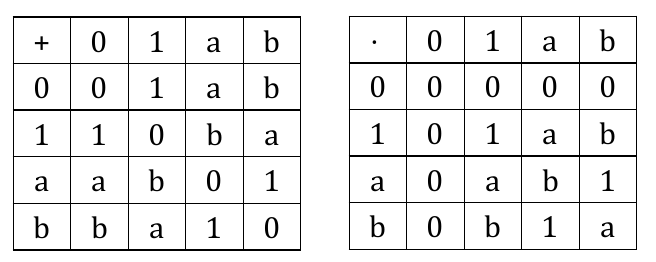
\includegraphics[scale=0.5]{images/tables}
	\caption{La table de $F_4$}
	\label{f4}
\end{wrapfigure}
On avait déjà vu le groupe $E_4$, qui comprend tous les éléments modulo 4. L'addition et multiplication sont définis normalement, simplement que $3+3 = 6 = 2$. Maintenant, on a $F_{p^m}$ seulement pour $p$ premier et $m$ entier. Par exemple, $F_4 = F_{2^2}$ On aura donc un groupe avec 4 éléments, mais répondant au modulo 2. Les tables de ce corps sont à droite. L'opération est une bijection ; on s'aide de cette information pour remplir le tableau (évident que $0+x = x$, et que $x+x = x(1+1) = x0 = 0$, mais difficile avec $a+b$). Les éléments se remplissent assez logiquement.

\subsubsection{Petit truc}
\begin{wrapfigure}{l}{6.4cm}
	\centering
	\captionsetup{justification=centering}
	\caption{Les tables de $F_4$ et de $\Z/2\Z^2$}
	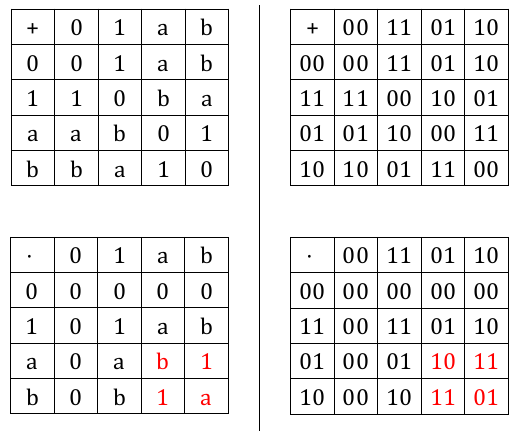
\includegraphics[scale=0.5]{images/tables_f4}
	\label{f4_z4}
\end{wrapfigure}
Pour l'addition, on peut tout a fait considérer $F_4$ comme $\Z/2\Z^2$ (deux éléments sur un modulo 2) ; mais la multiplication diffère un peu : si l'addition se comporte comme une addition standard ($xor$, sans retenue) sur deux bits, et la multiplication se comporte bizarrement : 00 met a 00, 11 ne change rien, et $01\times 01 = 10,\ 01\times 10 = 11$ et $10\times 10 = 01$. Donc attention !

Le tableau complet se trouve ci-contre, à la Figure \ref{f4_z4}

\subsection{(sous-)Ensemble vectoriel}
Soit $V$ un sous ensemble vectoriel  de $F_{p^m}^k$ ; il est engendré par plusieurs vecteurs de longueur $k$. Pour trouver la dimension du sous espace, on met les vecteurs dans une matrice et on réduit (attention à ne pas diviser) ; le nombre de colonnes pivots donne la \uline{dimension de $V$}, le \uline{cardinal} s'obtient avec $(p^m)^{dim(V)}$ (donc dimension 3 dans $F_{13}$ nous donnera un cardinal de $13^3$). On peut nous demander de trouver $p$, le nombre minimal d'équations pour engendrer $V$. Pour cela on reprend notre matrice réduite et on lui met comme solution 0. Ensuite on passe les éléments de l'autre côté, pour trouver la forme paramétrique. Attention, par le théorème du rang, il faut que $p + dim(V) = k$, donc que la dimension + le nombre de solutions = le nombre de variables/colonnes.

Résoudre les équations et réduire les matrices dans ces corps se fait d'une autre manière qu'on a l'habitude. Le but est toujours le même, mais au lieu de diviser on peut multiplier (dans $F_{13}$, pour "diviser" 8 par lui-même, il suffit de multiplier par 5)

\subsection{Espaces vectoriels}
Notons la \evid{Définition 12.3} des espaces vectoriels, importante :

Soit $\mathcal{K}$ un corps commutatif et $(\mathcal{V},\mathcal{+})$ un groupe commutatif, muni d'une opération binaire notée +. Supposons qu'une \uline{opération externe} est définie sur $\m{K}$ et $\m{V}$, c'est à dire une application qui à $\lambda \in \m{K}$ et $\vec{x} \in \m{V}$ associe un élément noté $\lambda\vec{x}$ de \m{V}. Les éléments du corps commutatif sont appelés \uline{scalaires} et les éléments de \m{V} sont appelés \uline{vecteurs}. L'opération externe est appelée \uline{multiplication scalaire} ou encore produit d'un vecteur par un scalaire. Nous disons que \m{V} muni de ces deux opérations es un \uline{espace vectoriel} sur le corps \m{K} si les propriétés suivantes sont vraies : pour tous scalaires $\lambda,\mu$ et vecteurs $\vec{u},\vec{v}$ :
\setstretch{1}
\begin{itemize}
	\item 	Associativité pour la multiplication scalaire : $\lambda(\mu \vec{v}) = (\lambda\mu)\vec{v}$
	\item 	Identité : $1\cdot\vec{v} = \vec{v}$
	\item 	Distributivité : $\lambda(\vec{u}+\vec{v}) = \lambda\vec{u} + \lambda\vec{v}$ et $(\lambda + \mu)\vec{v} = \lambda\vec{v} + \mu\vec{v}$
\end{itemize}
\setstretch{1.2}

\subsubsection{Sous-espace vectoriel}
Un sous-ensemble \m{S} de \m{V} ($\m{S} \subset \m{V}$) est un \uline{sous-espace vectoriel} s'il est aussi un espace vectoriel sur \m{K}. Cela revient à s'assurer que deux opérations sont définies :
\begin{equation*}
	\lambda\vec{u} \in \m{S} \text{ et } \vec{u} + \vec{v} \in \m{S} \qquad \forall \lambda \in \m{K},\ \vec{u},\vec{v} \in \m{S}
\end{equation*}
\begin{exemple}

	Considérons l'espace vectoriel $\F_7^3$ (donc l'ensemble des vecteurs représentés à la figure \ref{corps f37}) ainsi que l'ensemble \m{S} des vecteurs de la forme $(u,3u,6u)$. C'est un sous-espace vectoriel car 
	\begin{align*}
		\lambda(u,3u,6u) = \big(\lambda u,3(\lambda u),6(\lambda u)\big) \in \m{S}\\
		(u,3u,6u)+(v,3v,6v) = \big(u+v, 3(u+v) 6(u+v)\big)\in \m{S}
	\end{align*}
	Nous pouvons aussi considérer le sous-espace vectoriel \m{S}' des vecteurs $\vec{x} = (x_1,x_2,x_3)$ qui satisfont $x_1 + 4x_2 + 3x_3 = 0$ (c.f. exemple 12.5 du livre pour la preuve)
\end{exemple}
\begin{wrapfigure}{r}{4cm}
	\[\begin{pmatrix}
		0 & 0 & 0\\
		0 & 0 & 1\\
		\vdots & \vdots & \vdots\\
		0 & 0 & 6\\
		0 & 1 & 0\\
		\vdots & \vdots & \vdots\\
		6 & 6 & 6
	\end{pmatrix}\]
	\caption{Le corps $\F_7^3$}
	\label{corps f37}
\end{wrapfigure}
Notons également ces quelques termes : Une \uline{combinaison linéaire} de vecteurs $\vec{v}_i \in \m{V},\ i= 1\ldots m$ est une somme de la forme 
\begin{equation*}
	\vec{u} = \somme{m}{i=1} \lambda_i\vec{u}_i
\end{equation*}
où les c\oe fficients $\lambda_i$ sont des scalaires. L'ensemble des vecteurs $\vec{u}$ engendrés par toutes les combinaisons linéaires de $m$ vecteurs $v_1$ forme un sous espace vectoriel, appelé le \uline{sous-espace vectoriel engendré par les $\vec{v_i}$}.

Il sera parfois nécessaire de vérifier que des vecteurs sont \uline{linéairement indépendants}. Pour cela il suffit de réduire la matrice des vecteurs (selon la méthode du pivot de Gauss, vu en algèbre linéaire) ; les lignes non-nulles sont alors indépendantes entre elles. Ces vecteurs forment une \uline{base} de \m{V}. Cela signifie que l'ensemble des vecteurs de \m{V} peut s'écrire de manière unique comme une combinaison de ces vecteurs de la base ; les coefficients d'une telle combinaison s'appellent les \uline{coordonnées} du vecteur relativement à la base

\section[Codes linéaires]{Chapitre 13 : Les Codes Linéaires}
\begin{wrapfigure}{r}{3.7cm}	
	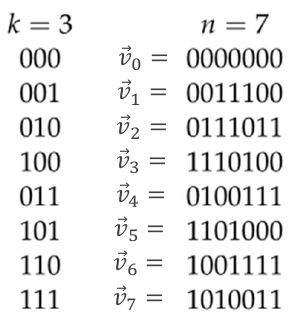
\includegraphics[scale=0.5]{images/code_C}
	\captionsetup{justification=centering}	
	\caption{Code C d'exemple}
	\label{code d'exemple}
\end{wrapfigure}
Pour les exemples, le code C de la Figure \ref{code d'exemple} sera utilisé.\\
\evid{Définition 13.1} :Soit C un code en bloc de longueur $n$. On dit que C est un \uline{code linéaire} si :
\setstretch{1}
\begin{enumerate}
	\item 	L'alphabet du code est un corps fini $K$
	\item 	Le code est un sous-espace vectoriel de $K^n$
\end{enumerate}
Cela ce traduit par la vérification de deux items (outre que l'alphabet est un corps fini) :
\begin{itemize}
	\item 	Si la somme de deux mots de code est encore un mot de code
	\item 	Si le vecteur nul ($\vec{0}$) est bien un mot de code
\end{itemize}
\setstretch{1.2}
\begin{exemple}[0.75]
	Est-ce que le code C est linéaire ?
	\begin{enumerate}
		\item 	L'alphabet est $F_2$, ce qui est un corps (fini)
		\item 	$v_4 = v_1 + v_2,\ v_5 = v_1+v_3,\ v_6 = v_2+v_3,\ v_7 = v_1+v_2+v_3$\\
				donc C est l'ensemble des 8 combinaisons linéaires de $v_1,v_2,v_3 \to$ OUI, c'est un code linéaire.
	\end{enumerate}
	On peut repérer si un code n'est pas linéaire par inspection (absence du vecteur nul ou si la somme de deux vecteurs n'est pas un mot), ou par taille : il est nécessaire qu'un code D-aire possède $D^k$ mots de code, pour un $k$ entier. Si un code binaire possède 3,5,6,... mots de code, c'est impossible, De même un code ternaire doit posséder 3,9,27,... mots de code.
\end{exemple}
\subsection{Dimension et distance minimale}
Soit \uline{$d$ = dimension du code linéaire} (= la dimension du sous-espace vectoriel des mots de code). Il y a $2^d$ mots de code, donc $k=d$ (k un des paramètres du code, c.f. Figure \ref{code d'exemple}).
\evid{Définition/Théorème 13.2 :} Si $K$ est un corps fini, le \uline{poids de Hamming} de $\vec{x} \in K^n$ est le nombre de composantes non-nulles, c'est à dire aussi $w(\vec{x}) \overset{\text{def}}{=} d(0,\vec{x})$.\\
La distance minimale d'un code linéaire C est égale à \[d_{min}(C) = \underset{\substack{\vec{x} \in C \\ \vec{x}\neq \vec{0}}}{\min}\, w(\vec{x})\]
\begin{exemple}
	Pour le code $C$, il y a 8 poids à calculer : $0,3,3,4,4,3,5,5$ (le nombre de \enquote{1} de chaque mot). Le minimum (outre 0) est 3, donc $d_{min}(C) = 3$
\end{exemple}
Notons bien que la distance à 0 est indépendante de la valeur non nulle de la coordonnée.
\begin{exemple}
	Pour un code dans $\F_7^3$, le mot 001 a une distance de 1, et le mot 111 a une distance de 3. Mais attention, car le mot 666 a aussi une distance de 3 et le mot 050 est de distance 1. On ne regarde pas la valeur de la composant, mais bien si elle est nulle ou pas.
\end{exemple}
\subsection{Matrice Génératrice}
\evid{Définition 13.3} Soit C un code linéaire sur le corps $K$, de longueur $n$ et dimension $k$. Soit ($\vec{v_1},\ldots,\vec{v_k}$) une base de C. La matrice obtenue en écrivant à la i-ième ligne le vecteur $\vec{v_i}$ est appelée une \uline{matrice génératrice du code}.

En gros, prendre la base (nombre minimal de vecteurs indépendants qui engendrent tous les autres mots) et les mettre dans une matrice.
\begin{exemple}
	On a vu que la base de C est constituée des vecteurs $(v_1,v_2,v_3)$. Donc la matrice génératrice 
	\[G = 
	\begin{pmatrix}
		0&0&1&1&1&0&0\\
		0&1&1&1&0&1&1\\
		1&1&1&0&1&0&0
	\end{pmatrix}
	\]
\end{exemple}
Cette matrice génératrice donne tous les mots de code. Donné un mot (pas encodé) $\vec{u}$, son encodage se trouve par $\vec{x} = \vec{u}\cdot G$
\begin{exemple}
	\[\vec{u} = (1,0,1) \to \vec{x} = \vec{u}G = (1,0,1)\cdot
	\begin{pmatrix}
		0&0&1&1&1&0&0\\
		0&1&1&1&0&1&1\\
		1&1&1&0&1&0&0
	\end{pmatrix}
	= 1,1,0,1,0,0,0\]
	Ce qui correspond au mot encodé, selon notre tableau (Figure \ref{code d'exemple})
\end{exemple}

\subsection{Forme Systématique}
\label{systematique}
La forme systématique d'une matrice est simplement sa forme échelonnée réduite. Le premier chiffre non nul de chaque ligne doit être un 1, et tous les éléments dans la colonne au dessus et au dessous de ce 1 doivent être nuls.

\begin{exemple}[0.5]
	Les deux matrices suivantes sont systématiques :
	\begin{center}
		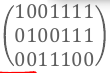
\includegraphics[scale=0.6]{images/g1}
		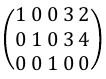
\includegraphics[scale=0.6]{images/g3}
	\end{center}	
\end{exemple}

\subsection{Matrice de contrôle}
\label{controle}
Le but de la matrice de contrôle est de vérifier qu'un séquence encodée soit valide, existe. Il faut donc réduire notre matrice G à une forme échelonnée (forme systématique) et exprimer les variables dépendantes telles que la somme vaut 0 ; \uline{il faut que $\vec{x}H^T = \vec{0}$}
\begin{exemple}
	Donnée la matrice génératrice 
	$\begin{pmatrix}
		0&1&2&3&4\\
		4&3&2&1&0\\
		1&1&0&1&1
	\end{pmatrix}$ dans $F_5$. Nous la réduisons comme nous savons le faire jusqu'à une forme symétrique : $\begin{pmatrix}
	1&0&0&3&2\\
	0&1&0&3&4\\
	0&0&1&0&0
	\end{pmatrix}$ Le code permet d'encoder des mots de 3 symboles $u_1u_2u_3$ à l'aide des formules (regarder les colonnes) :
	$\left\{\begin{array}{l}
	x_1 = u_1\\
	x_2 = u_2\\
	x_3 = u_3\\
	x_4 = 3u_1 + 3u_2\\
	x_5 = 2u_1 + 4u_2
	\end{array}\right.$\\
	 On prend nos deux dernières équations, et on les égalise à 0 :
	$\left\{\begin{array}{l}
	x_4-3x_1-3x_2 = 0\\
	x_5-2x_1-4x_2 = 0
	\end{array}\right. \to
	\left\{\begin{array}{l}
	2x_1+2x_2+x_4 = 0\\
	3x_1+x_2+x_5 = 0
	\end{array}\right.$ et il reste plus qu'à mettre en vecteurs et transposer :
	$(x_1,x_2,x_3,x_4,x_5)\cdot H^T = (\textbf{x}) \cdot \underbrace{\begin{pmatrix}
	2&3\\
	2&1\\
	0&0\\
	1&0\\
	0&1
	\end{pmatrix}}_{H^T} = (0,0)$
\end{exemple}
	Notons ainsi le théorème 13.1 :
	\begin{figure}[!h]
		\centering
		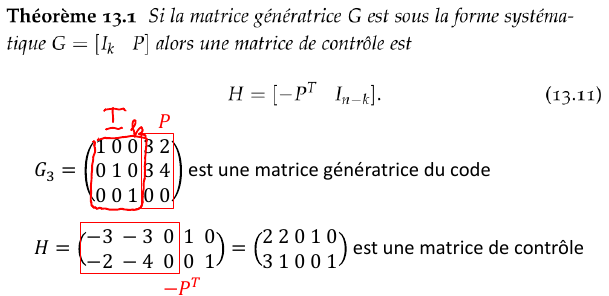
\includegraphics[scale=0.8]{images/theo13_1}
		\caption{Théorème 13.1 sur les matrices de contrôle}
	\end{figure}

\subsection{Syndrome}
\label{syndrome}
Soit $\vec{x} \in K^n$ un mot de $n$ symboles (\uline{pas nécessairement un mot de code}). Alors 
\[\vec{e}=\vec{x}H^T\]
s'appelle le \evid{syndrome}. Cela implique que
\[\vec{x} \text{ est un mot de code } \iff \vec{e} = \vec{x}H^T = \vec{0}\]
par définition de $H$.

\section[Codes de Reed-Solomon]{Chapitre 13 : Les Codes de Reed-Solomon}
Les codes de Reed-Solomon sont très utiles ; c'est le code le plus "efficace" pour encoder de l'information. Le code est linéaire (donc sur $F_{p^q},\ p$ premier et $q$ entier positif). Le rendement est variable ($r = \frac{k}{n}$ et on choisir $k,n$ tels que $k \leq n \leq p^q$). \uline{Ces codes atteignent \hyperref[Singleton]{la borne de Singleton} (ils sont MDS) par définition}
\subsection{Polynôme}
Prenons $\vec{u} = (u_1,u_2,\ldots,u_k) \in F^k$ pour certains champs finis F. Chaque $\vec{u}$ définit un polynôme $P_{\vec{u}}(x)$ (dans F) :
\begin{equation}
	P_{\vec{u}}(x) = u_1 + u_2x + u_3x^2 + u_4x^3 + \ldots + u_kx^{k-1}
	\label{P(u)}
\end{equation}
$P_{\vec{u}}(x)$ peut alors être évalué en tout $x \in F$\\
Le \evid{degré} du polynôme est la plus grande puissance de $x$ avec un coefficient non-nul.
\begin{exemple}
	Soit $F = F_5$ e $\vec{u} = (2,4,3).\ P_{\vec{u}}(x) = 2 + 4x + 3x^2$ et est de degré 2. Notons que $P(x) = 2$ (par exemple) est de degré 0 et que le degré de $P(x) = 0$ n'est pas défini (ou $-\infty$).
\end{exemple}

Nous savons, par le théorème 14.1 qu'un polynôme de degré $k-1$ (comme à l'équation \eqref{P(u)}) a au maximum $k-1$ solutions. S'il a $k$ solutions ou plus, alors $\vec{u} = \vec{0}$.
\begin{exemple}
	$x^2 - 3x + 2$ est de degré k-1 = 3-1 = 2, et a exactement 2 solutions : $x= 1$ et $x=2$.\\
	En revanche, $x^2 + 3x + 2$ n'a aucune solution.
\end{exemple}


\subsection{Construction du code}
La marche à suivre officielle se présente comme suit :\\
	\fcolorbox{black}{white}{
	\begin{minipage}{0.7\textwidth}
	Soient $n$ et $k$ des entiers avec $1 \leq k \leq n$. un code de Reed Solomon de paramètres $(n,k)$ est définit comme suit :
	\begin{enumerate}
		\item 	L'alphabet est un corps fini $K$ de cardinal $\geq n$
		\item 	Choisissons $n$ éléments distincts de $K, a_1,a_2,a_3,...,a_n$. Une suite de $k$ symboles $\vec{u} = (u_1,u_2,...,u_k) \in K^k$ est encodée en la suite de $n$ symboles $\vec{x} = (x_1,...,x_n) \in K^k$ définie par 
				\begin{equation*}
					x_i = P_{\vec{u}}(a_i) \quad \text{pour } i = 1,..,n
				\end{equation*}		 
	\end{enumerate}
	Le code de Reed Solomon C est l'ensemble de tous les encodages possibles, pour tous les $\vec{u} \in K^k$. C'est donc un code en bloc de longueur $n$.
	\end{minipage}}
\begin{exemple}
	\evid{En résumé :} On veut construire un code sur $F_5$. On doit choisir un $n$ entre 1 et 5, et un $k$ entre 1 et $n$. Prenons $n=5$ (maximum) et $k = 2$. Nous devons maintenant choisir 5 $a_i$. Comme nous devons choisir 5 éléments distincts dans $F_5$ nous n'avons pas le choix : $a_1 = 0,\ a_2 = 1,...,a_5 = 4$. Il faut maintenant encoder : on choisit tous les $\vec{u}$ (de longueur 2) possibles dans $F_5$. Par exemple, pour $\vec{u} = (3,2)$, alors $P_{\vec{u}}(X) = 3+2X$. Donc $P_{\vec{u}}(a_i) = 3 + 2\cdot a_i$. Toujours pour $\vec{u} = (3,2)$, nous obtenons 
	\begin{align*}
		P_{\vec{u}}(a_1) = P_{\vec{u}}(0) = 3\\
		P_{\vec{u}}(a_2) = P_{\vec{u}}(1) = 0\\
		P_{\vec{u}}(a_3) = P_{\vec{u}}(2) = 2\\
		P_{\vec{u}}(a_4) = P_{\vec{u}}(3) = 4\\
		P_{\vec{u}}(a_1) = P_{\vec{u}}(4) = 1
	\end{align*}
	et donc $\vec{x} = (3,0,2,4,1)$. Il faut répéter l'opération pour les $n^k$ suites.
\end{exemple}

\subsection{La matrice génératrice}
Un autre moyen de construire tous les mots de code est de passer par la matrice génératrice G. Pour cela, nous devons prendre une base de C, et donc $k$ vecteurs $\vec{u}$ linéairement indépendants. La manière la plus simple de créer G est de choisir des $\vec{u}$ qui formeront la $I_k$. Il ne reste alors plu qu'à créer $G$ selon ce tableau
	\[G = \begin{pmatrix}
	1 & 1 & 1 & 1 & 1\\
	a_1 & a_2 & a_3 & ... & a_n\\
	(a_1)^2 & (a_2)^2 & (a_3)^2 & ... & (a_n)^2\\
	... & ... & ... & ... & ...\\
	(a_1)^{k-1} & (a_2)^{k-1} & (a_3)^{k-1} & ... & (a_n)^{k-1}
	\end{pmatrix}\]
Cela s'explique facilement : le vecteur (1,0,0,0...,0) aura $P_{\vec{u}}(X) = 1$ donc une ligne remplie de 1. Le vecteur (0,1,0,0...,0) aura $P_{\vec{u}}(X) = X$ donc une ligne remplie de $a_1,a_2,a_3,...$. La suite continue : la 3\ts{ème} ligne sera (0,0,1,0,0,...,0) qui donnera $P_{\vec{u}}(X) = X^2$ donc une ligne remplie de $(a_i)^2$, etc. 	

La \hyperref[systematique]{forme systématique}, la \hyperref[controle]{matrice de contrôle} et le \hyperref[syndrome]{syndrome} se calculent comme précédemment.

\subsection[Notes/précisions sur Reed Solomon]{Notes et précisions sur les codes de Reed Solomon}
\begin{itemize}
	\item 	En choisissant les éléments $a_0,a_1,...$ dans un autre ordre que le naturel, le code sera toujours juste et le \enquote{même}, simplement que les mots seront dans un autre ordre.
	\item 	Pour corriger un mot qui a eu des effacements (pour autant que le poids de l'effacement soit \hyperref[canaux]{acceptable}), il suffit de chercher le syndrome du mot. Pour que le mot soit valide, le syndrome doit valoir 0. Cela nous donnera des équations, avec les effacements comme inconnues. Une simple résolution d'équations (avec des matrices par exemple) permet de trouver les effacements.
	\item 	Pour corriger les erreurs, c'est plus délicat à la main. Il faut connaître le poids de l'effacement. Chercher le syndrome du mot peut nous permettre de corriger avec un peu de jugeote. La série 12, exercice 6 donne une bonne méthode. Sinon allez exhaustivement : chercher toutes les corrections possibles et tester les syndromes.
\end{itemize}

\end{document} 